\chapter{Results}
\label{ch:chapter_4}

%% The following annotation is customary for chapter which have already been
%% published as a paper.
%\blfootnote{Parts of this chapter have been published in Annalen der Physik \textbf{324}, 289 (1906) \cite{Einstein1906}.}

%% It is only necessary to list the authors if multiple people contributed
%% significantly to the chapter.
%\authors{Albert {\titleshape Einstein}}

%% The '0pt' option ensures that no extra vertical space follows this epigraph,
%% since there is another epigraph after it.
%\epigraph[0pt]{
%    "quote1"
%}{attribution}

\epigraph{
    “No amount of experimentation can ever prove me right;
    
    a single experiment can prove me wrong. ”
}{Albert Einstein}

\begin{abstract}
Is this abstract enough?
\end{abstract}

%% Start the actual chapter on a new page.
\newpage
\section{Introduction}
While I have found the rather elegant many-body Green's Function (equation~\ref{eq:mbgfresult}), this does not tell us what the exact predictions are as they largely depend on the particular system or molecule.

In \citet{perrinnano}, the authors found a pronounced Negative-Differential Conductance (NDC) which is readily explained from a two site model, which I present here. Note that while the NDC was qualitatively explained by the two-site model, they used a prefactor $7.2 \times 10^{-5}$ to match the absolute values of the current. This has yet to be explained, and the Coulomb interaction was our prime suspect. The explanation lies in that the bias window usually encompasses only a single transmission peak, which is suppressed due to the Stark effect. As a result, the current first peaks before it is suppressed, leading to the NDC. Note that if no peak is in the bias-window at $V\ll1$, the current shape will have a plateau around $V=0$ which extends until a transmission peak enters the bias window. 

In section~\ref{sec:twosite}, I define the model both with and without spin. I consider some general characteristics and expectations under the approximation that the many-body states are Boltzmann distributed in section~\ref{sec:expectations}. I then look at the transmission functions in section~\ref{sec:twositetransmission}. The $I(V)$ characteristics for selected parameter sweeps are presented in section~\ref{sec:twositeparamsweep}. The improvement on quantitative agreement with the experiment of Ref.~\cite{perrinnano} is shown in section~\ref{sec:perrin}. Finally, in section~\ref{sec:resultsselfconsistent} I present some results that make use of the self-consistency ( equation~\ref{eq:selfconsistency}) in section~\ref{sec:resultsselfconsistencycalc}.


\section{Two site model} 
The model comes in two flavors; with and without spin. 
\label{sec:twosite}
\subsection{Spinless two site model}
The form of the two-site model including Stark effect has been confirmed with DFT calculations in the supplement of Ref.~\cite{perrinnano}. I  will first look at the model without including spin. The Hamiltonian including tunnelling terms is:
\begin{align}
H_1 &= \begin{bmatrix} \epsilon_0 + \frac{1}{2} \alpha V & -\tau \\
-\tau & \epsilon_0 - \frac{1}{2} \alpha V\end{bmatrix},
\label{eq:spinlesshamiltonian}
\end{align}
where $\epsilon_0$ is the zero-bias level, $\tau$ is the tunnelling strength, $\alpha$ is the bias-level coupling due to the Stark effect and $V$ is the bias Voltage (in eV). The molecule is assumed to couple symmetrically to the left and right leads in the WBL:
\begin{align*}
\Gamma^L &= \begin{bmatrix} \Gamma & 0 \\ 0 & 0 \end{bmatrix},\\ \Gamma^R &= \begin{bmatrix} 0 & 0 \\ 0 & \Gamma \end{bmatrix},
\end{align*}
where $\Gamma$ is the molecule-lead coupling strength. The capacitive self-energy (equation~\ref{eq:selfenergycapacitive}) is given by:
\begin{align*}
\Sigma^c &= \begin{bmatrix} U & 0 \\ 0 & 0 \end{bmatrix} n_2 + \begin{bmatrix} 0 & 0 \\ 0 & U \end{bmatrix} n_1,
\end{align*}
where $U$ is the capacitive interaction strength.  The model is depicted schematically in Figure~\ref{fig:twosite}, where I have explicitly drawn the capacitive interaction. The leads are at different heights due to applied bias. In this model, where capacitive interaction is between two electrons instead of the electrons and the entire molecular background, the capacitive interaction is just the Coulomb Interaction\footnote{As previously indicated in section~\ref{sec:mbgfno}, there are molecules for which the interaction term is slightly more complicated and we can directly get the results from a number of DFT calculations.}.


\begin{figure}[htb]
    \begin{subfigure}[b]{0.48\textwidth}
        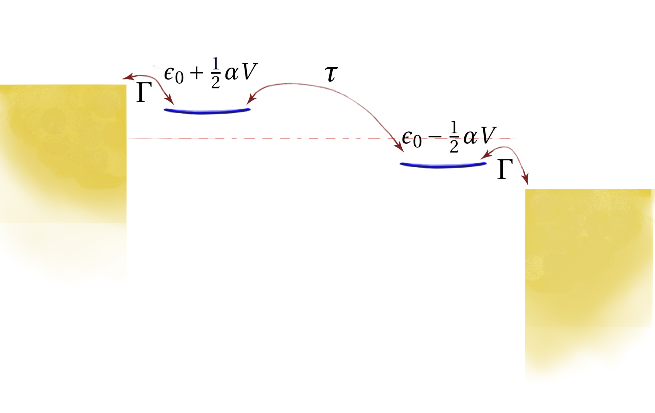
\includegraphics[height=.20\textheight]{pdf/non_interacting_schematics.pdf}\caption{non\hyp{}interacting}\label{fig:twositea}
    \end{subfigure}
    ~
    \begin{subfigure}[!tb]{0.48\textwidth}
        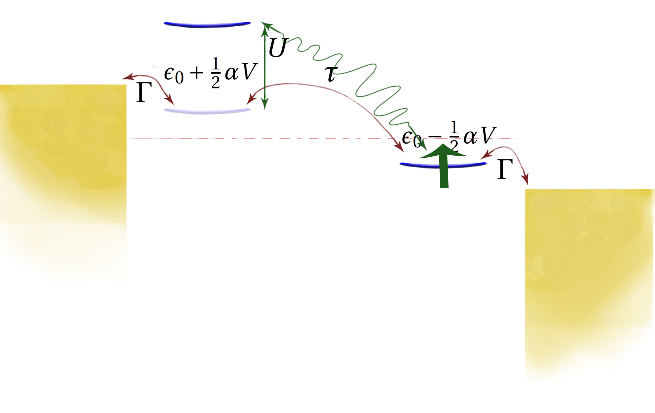
\includegraphics[height=.20\textheight]{pdf/interacting_schematics.pdf}\caption{Interacting}\label{fig:twositeb}
    \end{subfigure}
    \caption{Schematic pictures of the spinless two site model. The red dashed line denotes the Fermi-level. Figure~\ref{fig:twositea} shows the non\hyp{}interacting case, where $\Gamma$ is the molecule-lead coupling, $\epsilon \pm \frac{1}{2} \alpha V$ are the left (right) level and $\tau$ is the tunnelling strength between the levels. In Figure~\ref{fig:twositeb}, an electron (large green arrow) occupies the right level. The swirly line is meant to indicate an interaction with electrons on the left level, thereby raising the level with the capacitive interaction or charging energy $U$.} \label{fig:twosite}
\end{figure}

When no capacitive interaction is included (i.e. $U=0$), the common method (section~\ref{sec:synthesis}) can be applied to find the transmission analytically: \cite{perrinnano}\footnote{If the bias voltage is assumed to be distributed symmetrically over the leads, then the current can be found analytically as well. However, this serves no purpose in this discussion.}:
\begin{align*}
T(\epsilon) &= \frac{ (2\tau)^2 }{(\frac{\Gamma}{2})^2} \frac{(\frac{\Gamma}{2})^2}{(\epsilon-\epsilon_1)^2 + (\frac{\Gamma}{2})^2}\frac{(\frac{\Gamma}{2})^2}{(\epsilon-\epsilon_2)^2 + (\frac{\Gamma}{2})^2},
\end{align*}
where $\epsilon_{1,2} = \epsilon_0 \pm \frac{1}{2} \Delta$, where $\Delta$ is the level splitting in the presence of bias voltage given by $\Delta = \sqrt{ (\alpha V)^2+ 4\tau^2}$. 

For the two-site model including capacitive interactions, we assume that the chance a many-body state $\ket{\kappa}$ is occupied is proportional to the Boltzmann-factor $e^{ -\beta \braket{ \kappa\left| H \right| \kappa}} Z^{-1}$, where $Z$ is a normalisation constant and $H$ the full Hamiltonian including capacitive interactions.

It is illustrative for the application of the many-body Green's function (equation~\ref{eq:mbgfresult}) to consider the shapes of $G^{\lambda\pm}$. Their most important contribution in this context is simply the thermal average of the capacitive self-energy $\braket{\lambda\left|\Sigma^c\right|\lambda}$. The four $G^{\lambda\pm}$ are:
\begin{align*}
G^{\ket{00}\pm} &= \left[ \epsilon \begin{bmatrix} 1 & 0 \\ 0 & 1 \end{bmatrix} - \begin{bmatrix} \epsilon_0 + \frac{1}{2} \alpha V & -\tau \\
-\tau & \epsilon_0 - \frac{1}{2} \alpha V\end{bmatrix}  \pm \frac{\imath}{2} \begin{pmatrix} \Gamma & 0 \\ 0 & \Gamma \end{pmatrix} \right]^{-1}, \\
G^{\ket{10}\pm} &= \left[ \epsilon \begin{bmatrix} 1 & 0 \\ 0 & 1 \end{bmatrix} - \begin{bmatrix} \epsilon_0 + \frac{1}{2} \alpha V & -\tau \\
-\tau & \epsilon_0 - \frac{1}{2} \alpha V\end{bmatrix} - \begin{pmatrix} 0 & 0 \\ 0 & U \end{pmatrix} \pm \frac{\imath}{2} \begin{pmatrix} \Gamma & 0 \\ 0 & \Gamma \end{pmatrix} \right]^{-1}, \\
G^{\ket{01}\pm} &= \left[ \epsilon \begin{bmatrix} 1 & 0 \\ 0 & 1 \end{bmatrix} - \begin{bmatrix} \epsilon_0 + \frac{1}{2} \alpha V & -\tau \\
-\tau & \epsilon_0 - \frac{1}{2} \alpha V\end{bmatrix} - \begin{pmatrix} U & 0 \\ 0 & 0 \end{pmatrix} \pm \frac{\imath}{2} \begin{pmatrix} \Gamma & 0 \\ 0 & \Gamma \end{pmatrix} \right]^{-1},\\
G^{\ket{11}\pm} &= \left[ \epsilon \begin{bmatrix} 1 & 0 \\ 0 & 1 \end{bmatrix} - \begin{bmatrix} \epsilon_0 + \frac{1}{2} \alpha V & -\tau \\
-\tau & \epsilon_0 - \frac{1}{2} \alpha V\end{bmatrix} - \begin{pmatrix} U & 0 \\ 0 & U \end{pmatrix} \pm \frac{\imath}{2} \begin{pmatrix} \Gamma & 0 \\ 0 & \Gamma \end{pmatrix} \right]^{-1},
\end{align*}
where we see that adding an electron to e.g. $\ket{10}$ would add the energy $\epsilon_2$ and the capacitive interaction energy $U$. We see this quite clearly in the capacitive self-energy contribution of $G^{\ket{10}\pm}$. 

\subsection{Spinfull two site model}
When we include spin in the model, we are essentially keeping two copies of the model and add interaction. There is no spin-flip tunnelling. I use the ordered many-body basis $\left\{ \ket{\uparrow 1}, \ket{\downarrow 1}, \ket{\uparrow 2}, \ket{\downarrow 2}\right\}$. The Hamiltonian is:
\begin{align}
H_1 &= \begin{bmatrix} \epsilon_0 + \frac{1}{2} \alpha V & 0 & -\tau & 0 \\ 0 & \epsilon_0 + \frac{1}{2} \alpha V & 0 & -\tau\\ -\tau & 0 & \epsilon_0 - \frac{1}{2} \alpha V & 0 \\ 0 & -\tau & 0 & \epsilon_0 - \frac{1}{2} \alpha V\end{bmatrix},
\label{eq:spinfullhamiltonian}
\end{align} 
while the coupling matrices are:
\begin{align*}
\Gamma^L &= \begin{bmatrix} \Gamma & 0 & 0 & 0 \\ 0 & \Gamma & 0 & 0 \\ 0 & 0 & 0 & 0 \\  0 & 0 & 0 & 0\end{bmatrix},\\ \Gamma^R &= \begin{bmatrix} 0 & 0 & 0 & 0 \\ 0 & 0 & 0 & 0 \\ 0 & 0 & \Gamma & 0 \\ 0 & 0 & 0 & \Gamma \\ \end{bmatrix},
\end{align*}
and the capacitive self-energy is:
\begin{align*}
\Sigma^c &= \begin{bmatrix} \zeta U & 0 & 0 & 0\\ 0 & \zeta U & 0 & 0\\ 0 & 0 & 0 & 0\\ 0 & 0 & 0 & \xi U \end{bmatrix} n_{\uparrow 2} + \begin{bmatrix} \zeta U & 0 & 0 & 0\\ 0 & \zeta U & 0 & 0\\ 0 & 0 & \xi U & 0\\ 0 & 0 & 0 & 0 \end{bmatrix} n_{\downarrow 2} +\\
&\quad\begin{bmatrix} 0 & 0 & 0 & 0\\ 0 & \xi  U & 0 & 0\\ 0 & 0 & \zeta U & 0\\ 0 & 0 & 0 & \zeta U \end{bmatrix} n_{\uparrow 1} + \begin{bmatrix} \xi  U & 0 & 0 & 0\\ 0 & 0 & 0 & 0\\ 0 & 0 & \zeta U & 0\\ 0 & 0 & 0 & \zeta U \end{bmatrix} n_{\downarrow 1},
\end{align*}
where $\zeta U$ describes the strength of capacitive interaction between the left and right site (intersite), whereas $\xi U$ describes the strength of capacitive interaction on the left or right site (onsite).

The definitions for the coupling matrices $\Gamma^{R,L}$ allow us to directly calculate the transmission analytically in terms of the retarded and advanced Green's Function \emph{if only a single state is occupied}:
\begin{align*}
T(\epsilon) &= \Gamma^2 \left( G^+_{13} G^-_{31} + G^+_{14} G^-_{41} + G^+_{23} G^-_{32} + G^+_{24} G^-_{42} \right),
\end{align*}
where $\Gamma$ is the WBL coupling constant.Note that there is in principle a maximum of $4$ peaks. Because $\left(G^+\right)_{ij}^\star = G^-_{ji}$ in the energy-domain, there is no quantum interference and the function is real valued, as it should be. If the energy state is degenerate, the $G^\pm \rightarrow \mathscr{G}^\pm$ and quantum interference is possible.

\section{Expectations}
\label{sec:expectations}
Expectations for both flavors (spinless, spinfull) are discussed. 
\subsection{Spinless two-site model}
In section~\ref{sec:twositetransmission}, I will look at selected transmission figures for $U=0.0, 0.05, 0.15$ and $0.5$. The many-body character of the new theory makes it imperative to look at the many-body energies before I can make predictions about the different figures.

The initial guess for the self-consistency procedure (equation~\ref{eq:selfconsistency}) starts with the Boltzmann distribution as an initial guess, which specifies that only the lowest-energy many-body state is occupied. However, due to time constraints I have not used the self-consistency procedure, only working with the initial guess.

I conferred with Jose Celis Gil, and we agreed that the low temperature energy scale compared to the energy scales of the single-particle levels would cause rapid dissipation, implying a near\hyp{}equilibrium state, thereby justifying the approximation to the many-body occupation probabilities. Nevertheless, we did check this assumption. In Figure~\ref{fig:occprob}, we see that the self-consistent occupation probabilities (coloured diamonds) differ from the Boltzmann distribution (dashed lines) for $\left|V\right|\lesssim 0.10$. The theoretical mismatch of peak current in Ref.~\cite{perrinnano} has peaks at $\left|V\right|\approx 0.05$, so that the mismatch in occupation probabilities is only significant when no transmission peaks aligns with the Fermi-level. The mismatch is small when the levels start aligning, but seems sufficiently small that approximating by the Boltzmann distribution seems justifiable. In section~\ref{sec:resultsselfconsistencycalc}, I present a result that makes use of the self-consistency equation.

\begin{figure}[htb]
    \centering
    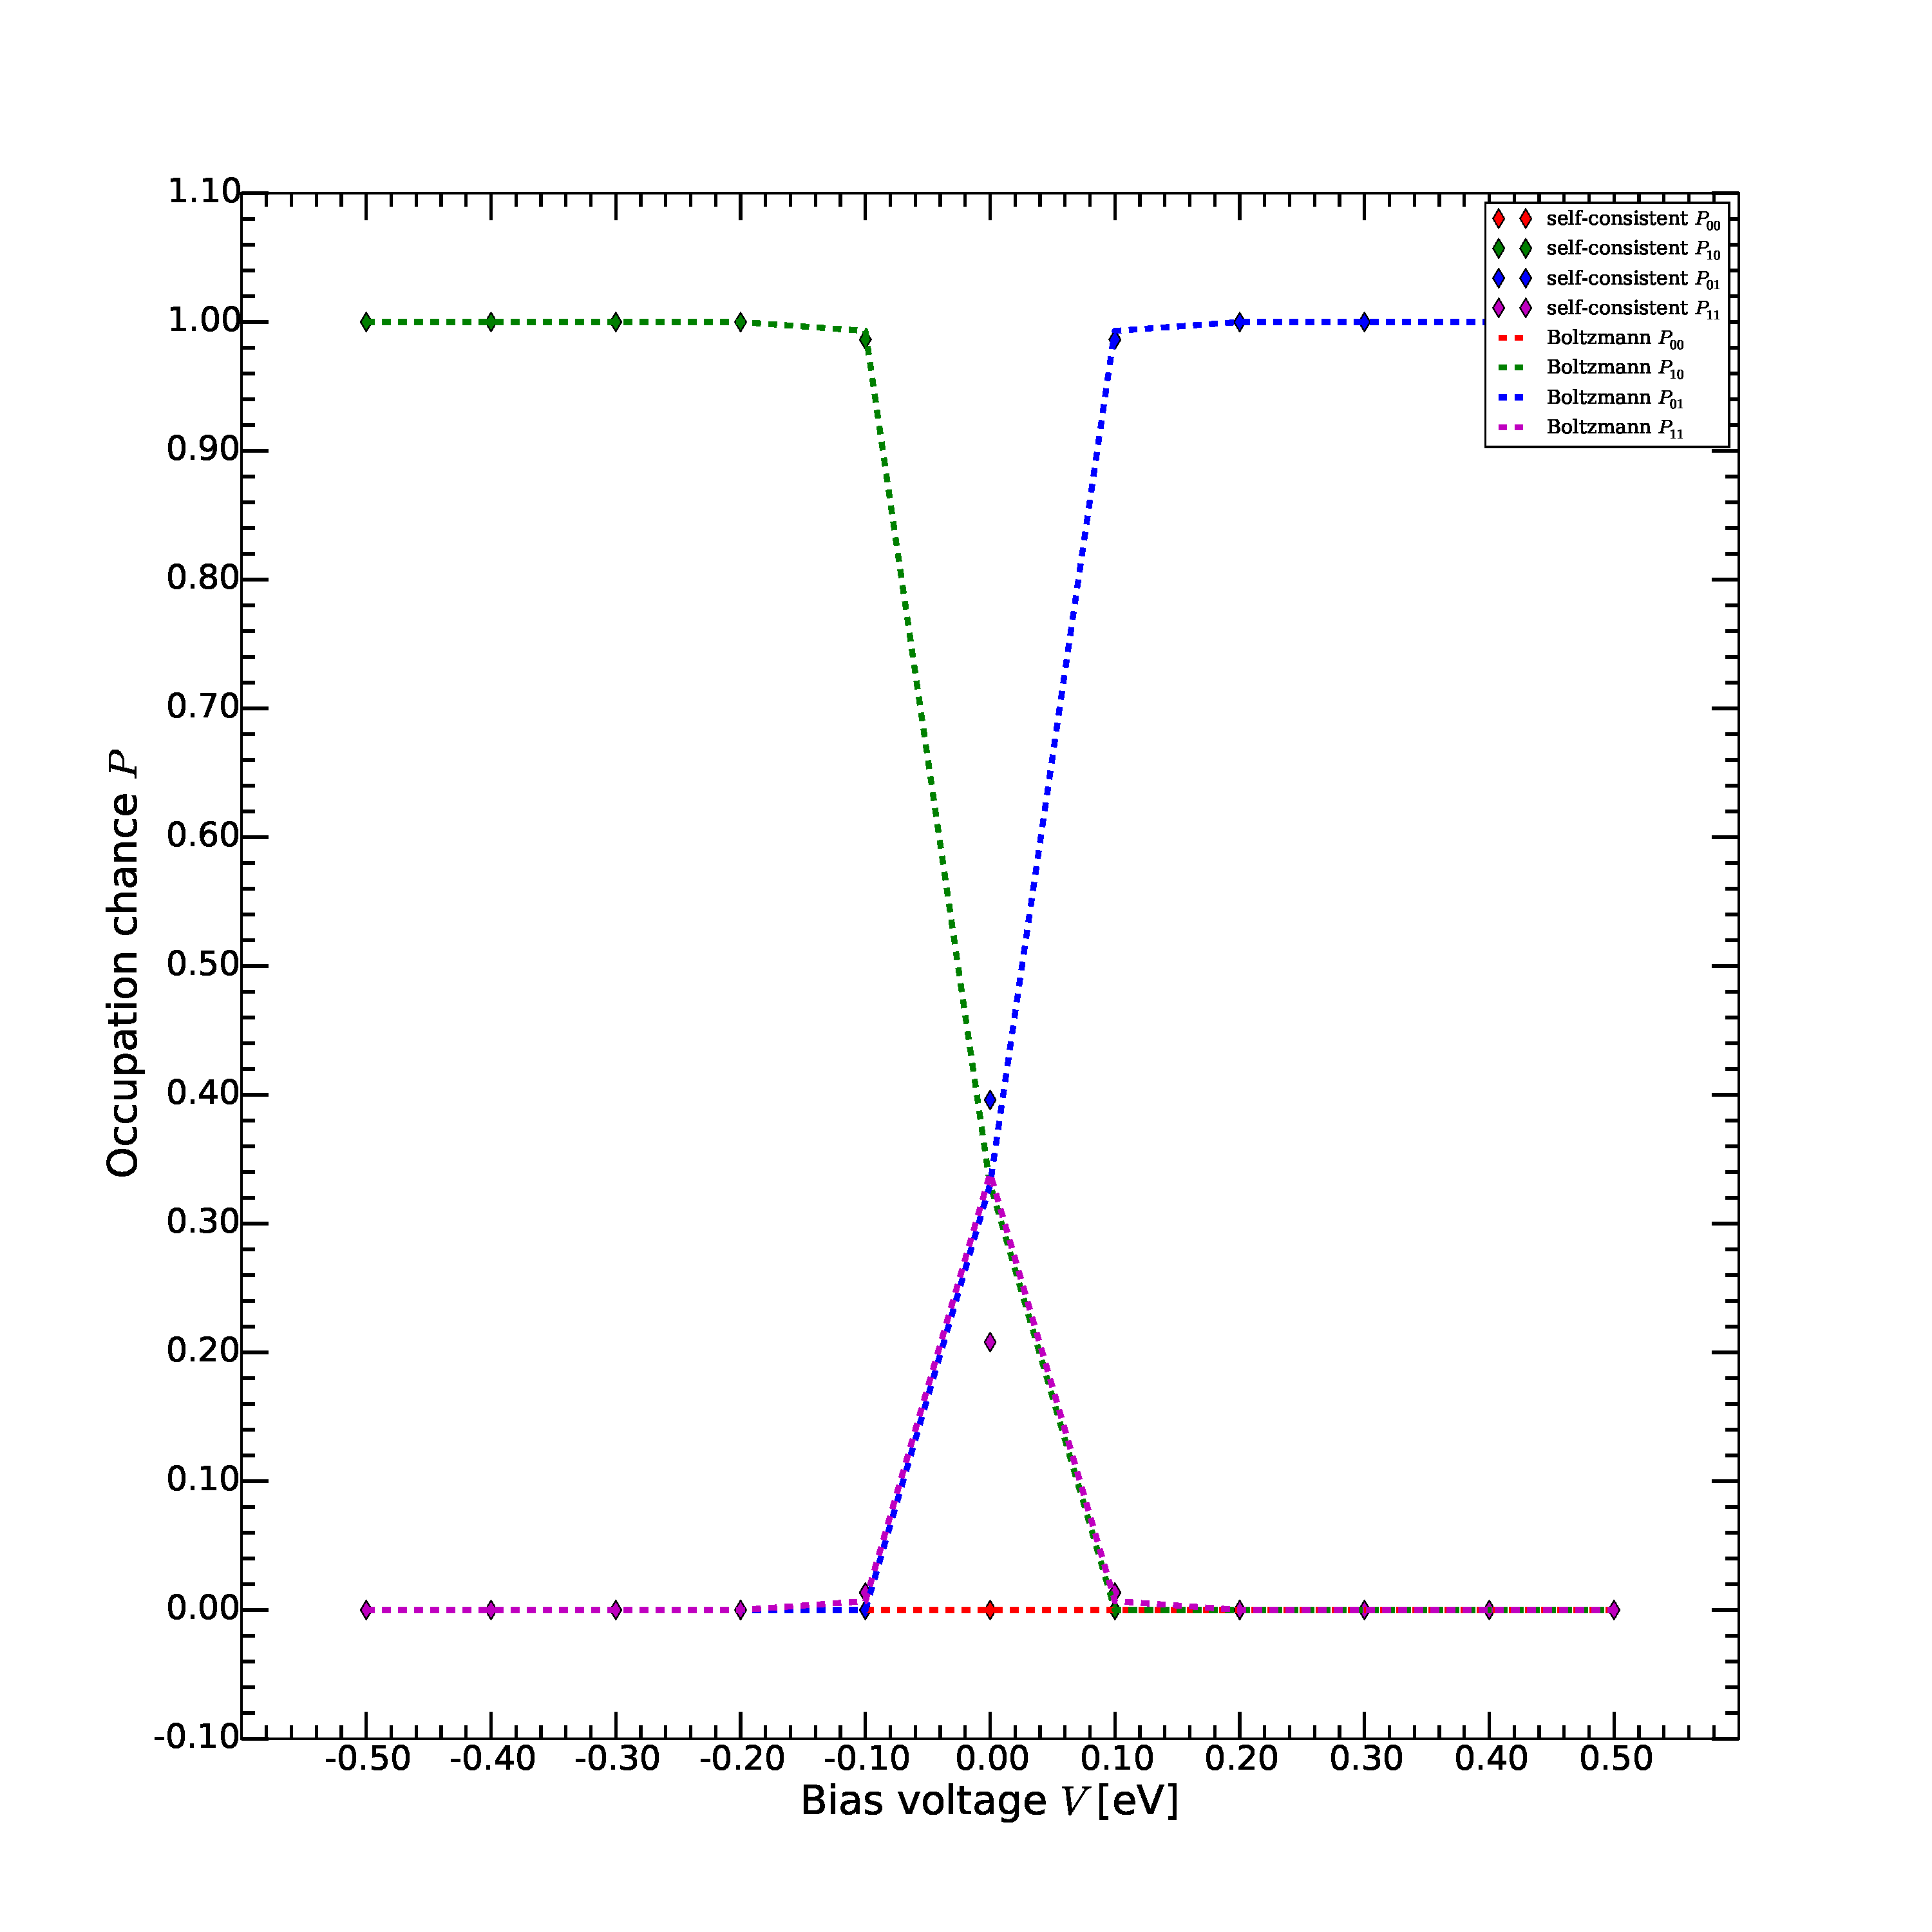
\includegraphics[width=.95\textwidth]{pdf/selfconsistent_low_temperature_1.pdf}
    \caption{Occupation probabilities $P_\kappa$ found by the self-consistency procedure (equation~\ref{eq:selfconsistency}) versus potential difference $V$ (coloured diamonds). The self-consistent results differ slightly from the Boltzmann distribution (dashed lines) around $V=0$, but do not differ from the Boltzmann distribution for $\left|V\right|\gtrsim 0.10$.}
    \label{fig:occprob}
\end{figure} \clearpage

Figure~\ref{fig:perrinenergy1} with $U=0.05$ is of interest because it shows the many-body character of my calculation, because the capacitive interaction enables the switch from $\ket{01}$ to $\ket{11}$ , which also causes a switch in transport behaviour. In the first state, there will be one transmission peak at $\epsilon_R$ and one at $\epsilon_L + U$. However, in the second state the second peak is also raised to $\epsilon_R+U$. Since this moves the levels further off-resonance, the transmission peak will be of lower height. 
\begin{figure}[htb]
    \centering
    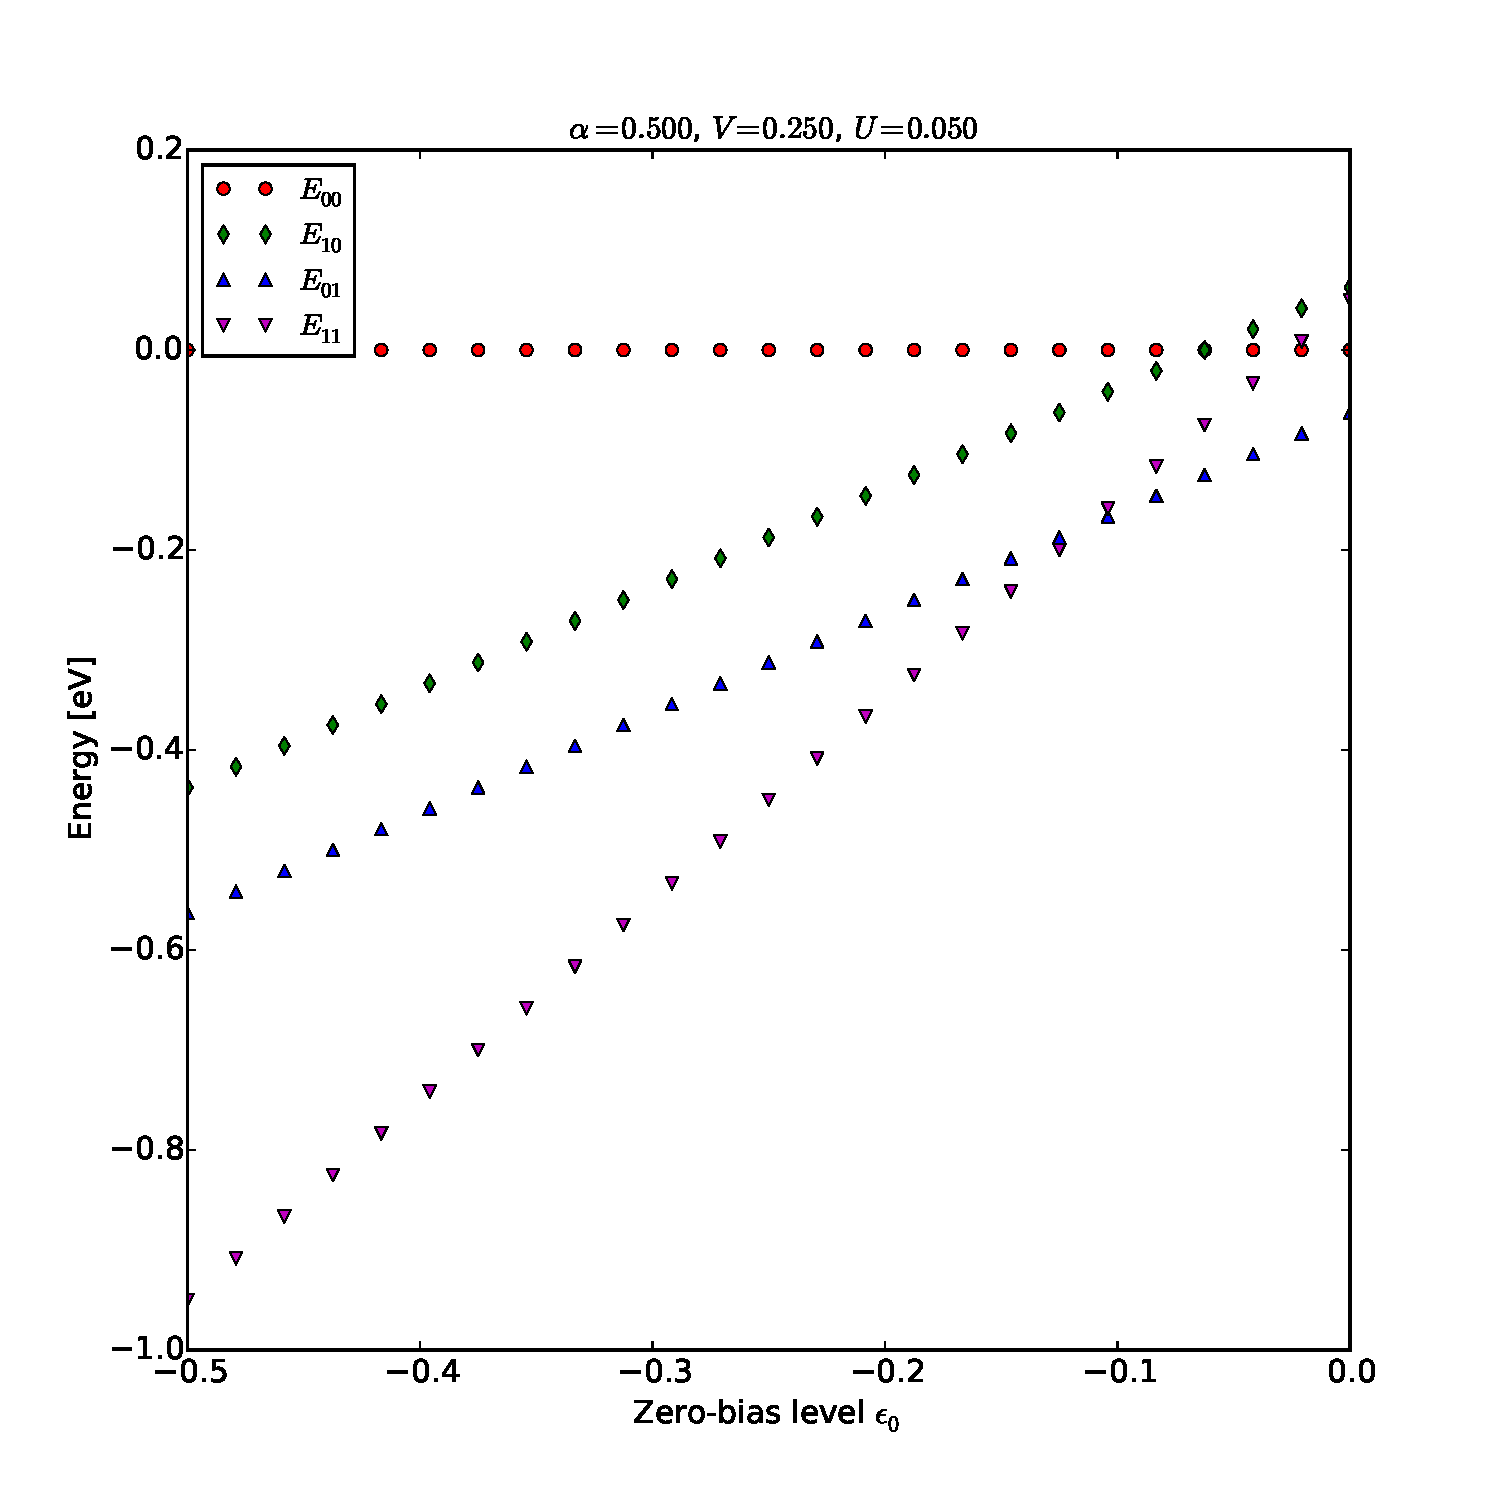
\includegraphics[height=.45\textheight]{pdf/energy/perrin_distribution_u1.pdf}
    \caption{Energy of many-body states versus zero-bias level $\epsilon_0$ for the spinless two-site model at $U=0.05$. The subscripts $E_{ij}$ refer to the many-body state $\ket{i j}$. At $\epsilon_0 \approx 0$, there is one electron on the right level. Lowering $\epsilon_0$ past ~$-0.12$ indicates a shift to an occupation of both the left and right levels.  }
    \label{fig:perrinenergy1}
\end{figure} 

 
\subsection{Spinfull two-site model} 
In this section, I present the energies of the spinfull model for $U=0.05$, $\zeta=1.00$, $\xi=1.00$, parameters that to match the transmission figure presented in section~\ref{sec:twositetransmission}.
 
\begin{figure}[htb]
    \centering
    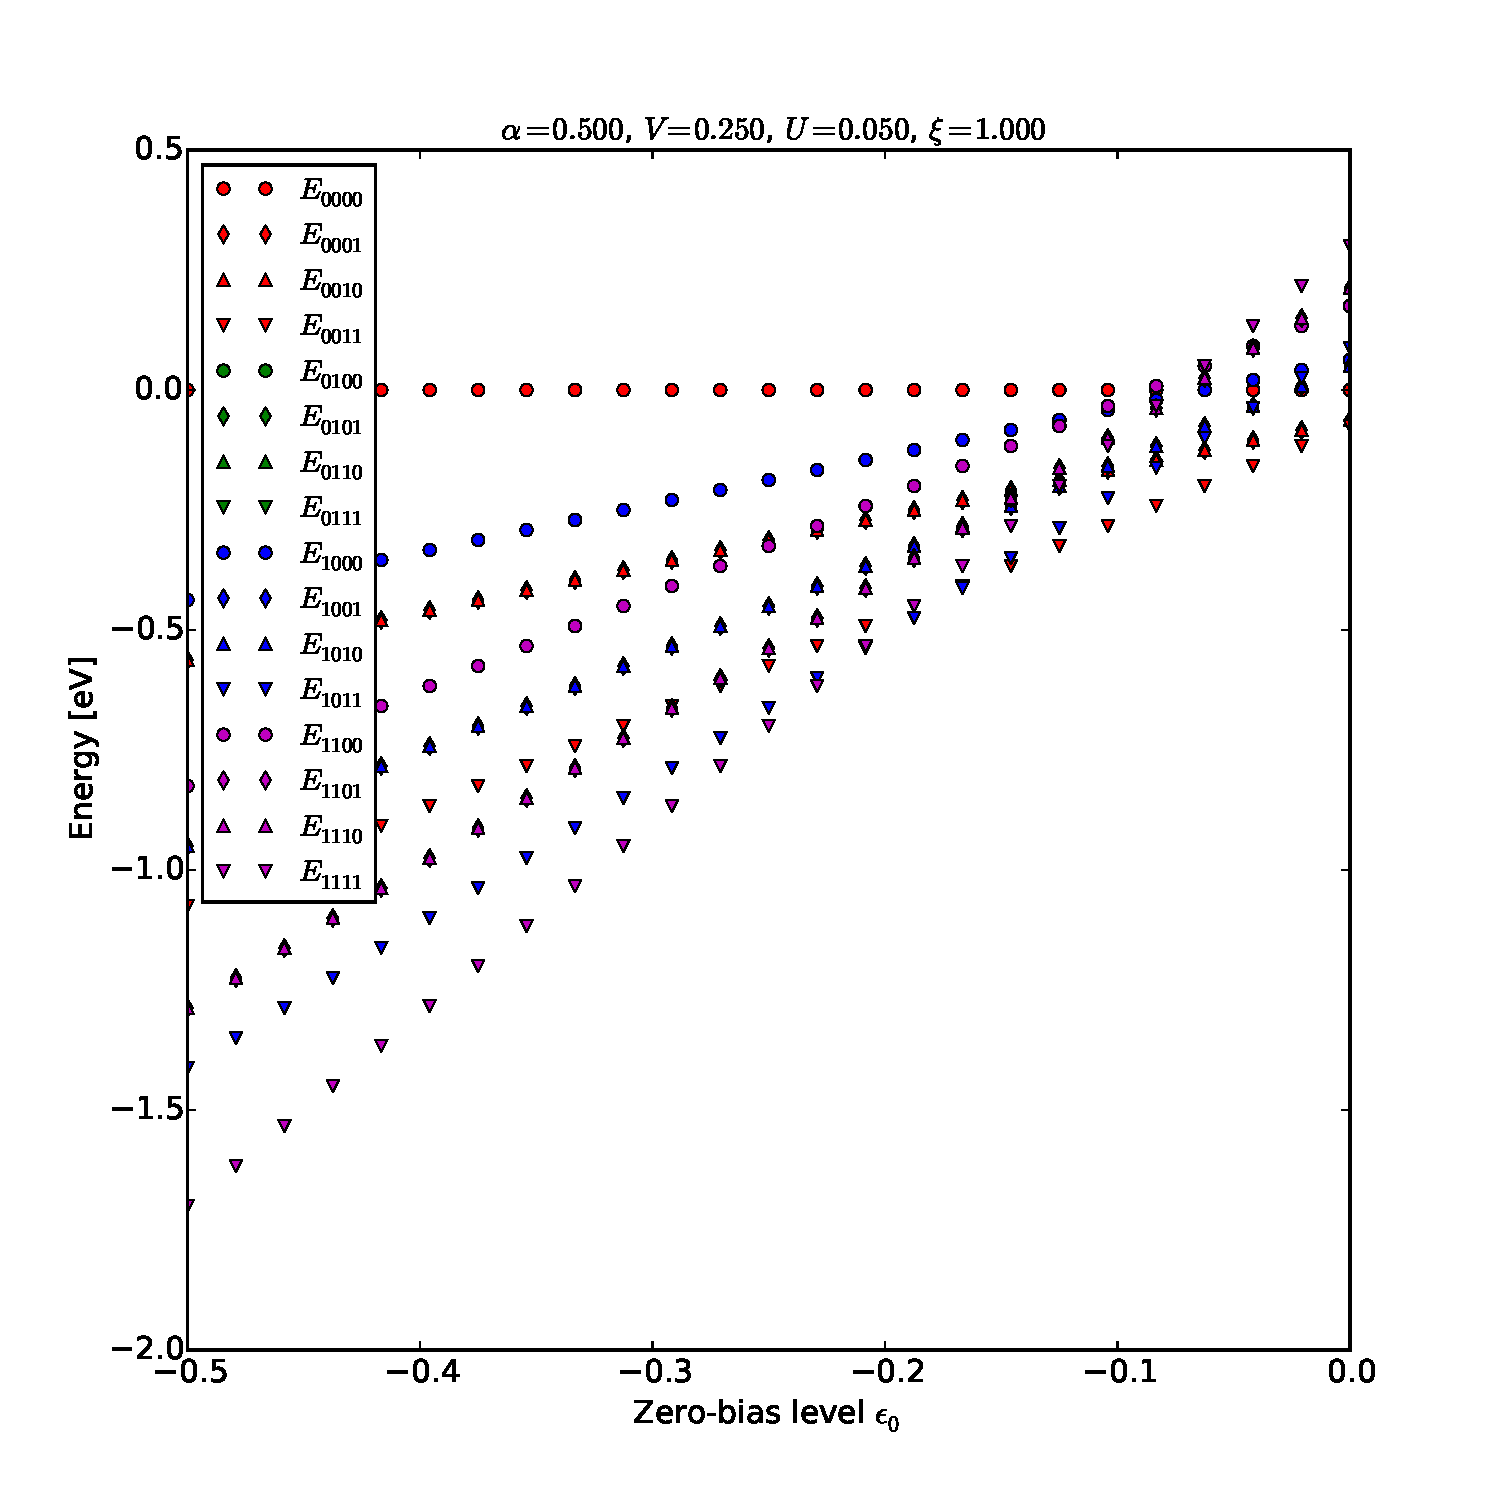
\includegraphics[height=.45\textheight]{pdf/energy/pespin_distribution_u1_k2.pdf}
    \caption{Energy of many-body states versus zero-bias level $\epsilon_0$ for the spinfull two-site model. In this figure, $U=0.05$, $\zeta=1.00$, $\xi=1.00$. The lowest energy state is $\ket{0011}$ for $\epsilon_0\gtrsim -0.15$, which then switches to $\ket{1011}$ before switching to $\ket{1111}$ at $\epsilon_0 \lesssim -0.20$.}
    \label{fig:perspinenergy12}
\end{figure}  


The Fock-space of occupation states for the spinfull model has dimension $2^4$, so that there are that many energies in the figures. In Figure~\ref{fig:perspinenergy12} I see similar behaviour as in the spinless case. There are switches between different many-body states, which are expected to cause some transmission peaks to shift by $\zeta U$ or $\xi U$ or both. The specifics of the many-body states are indicated in their captions.
\section{Transmission}
\label{sec:twositetransmission}
Transmissions for both flavors (spinless, spinfull) are discussed. 
\subsection{Spinless two-site model}
First, I want to look at the transmission for the spinless model.Figure~\ref{fig:spinlesstransmission} compares an interacting ($U=0.5$) transmission spectrum versus a non-interacting one. The effect of interaction is apparently to suppress the transmission peak height and move the rightmost peak outwards by $U$. 
\begin{figure}[htb]
    \centering
    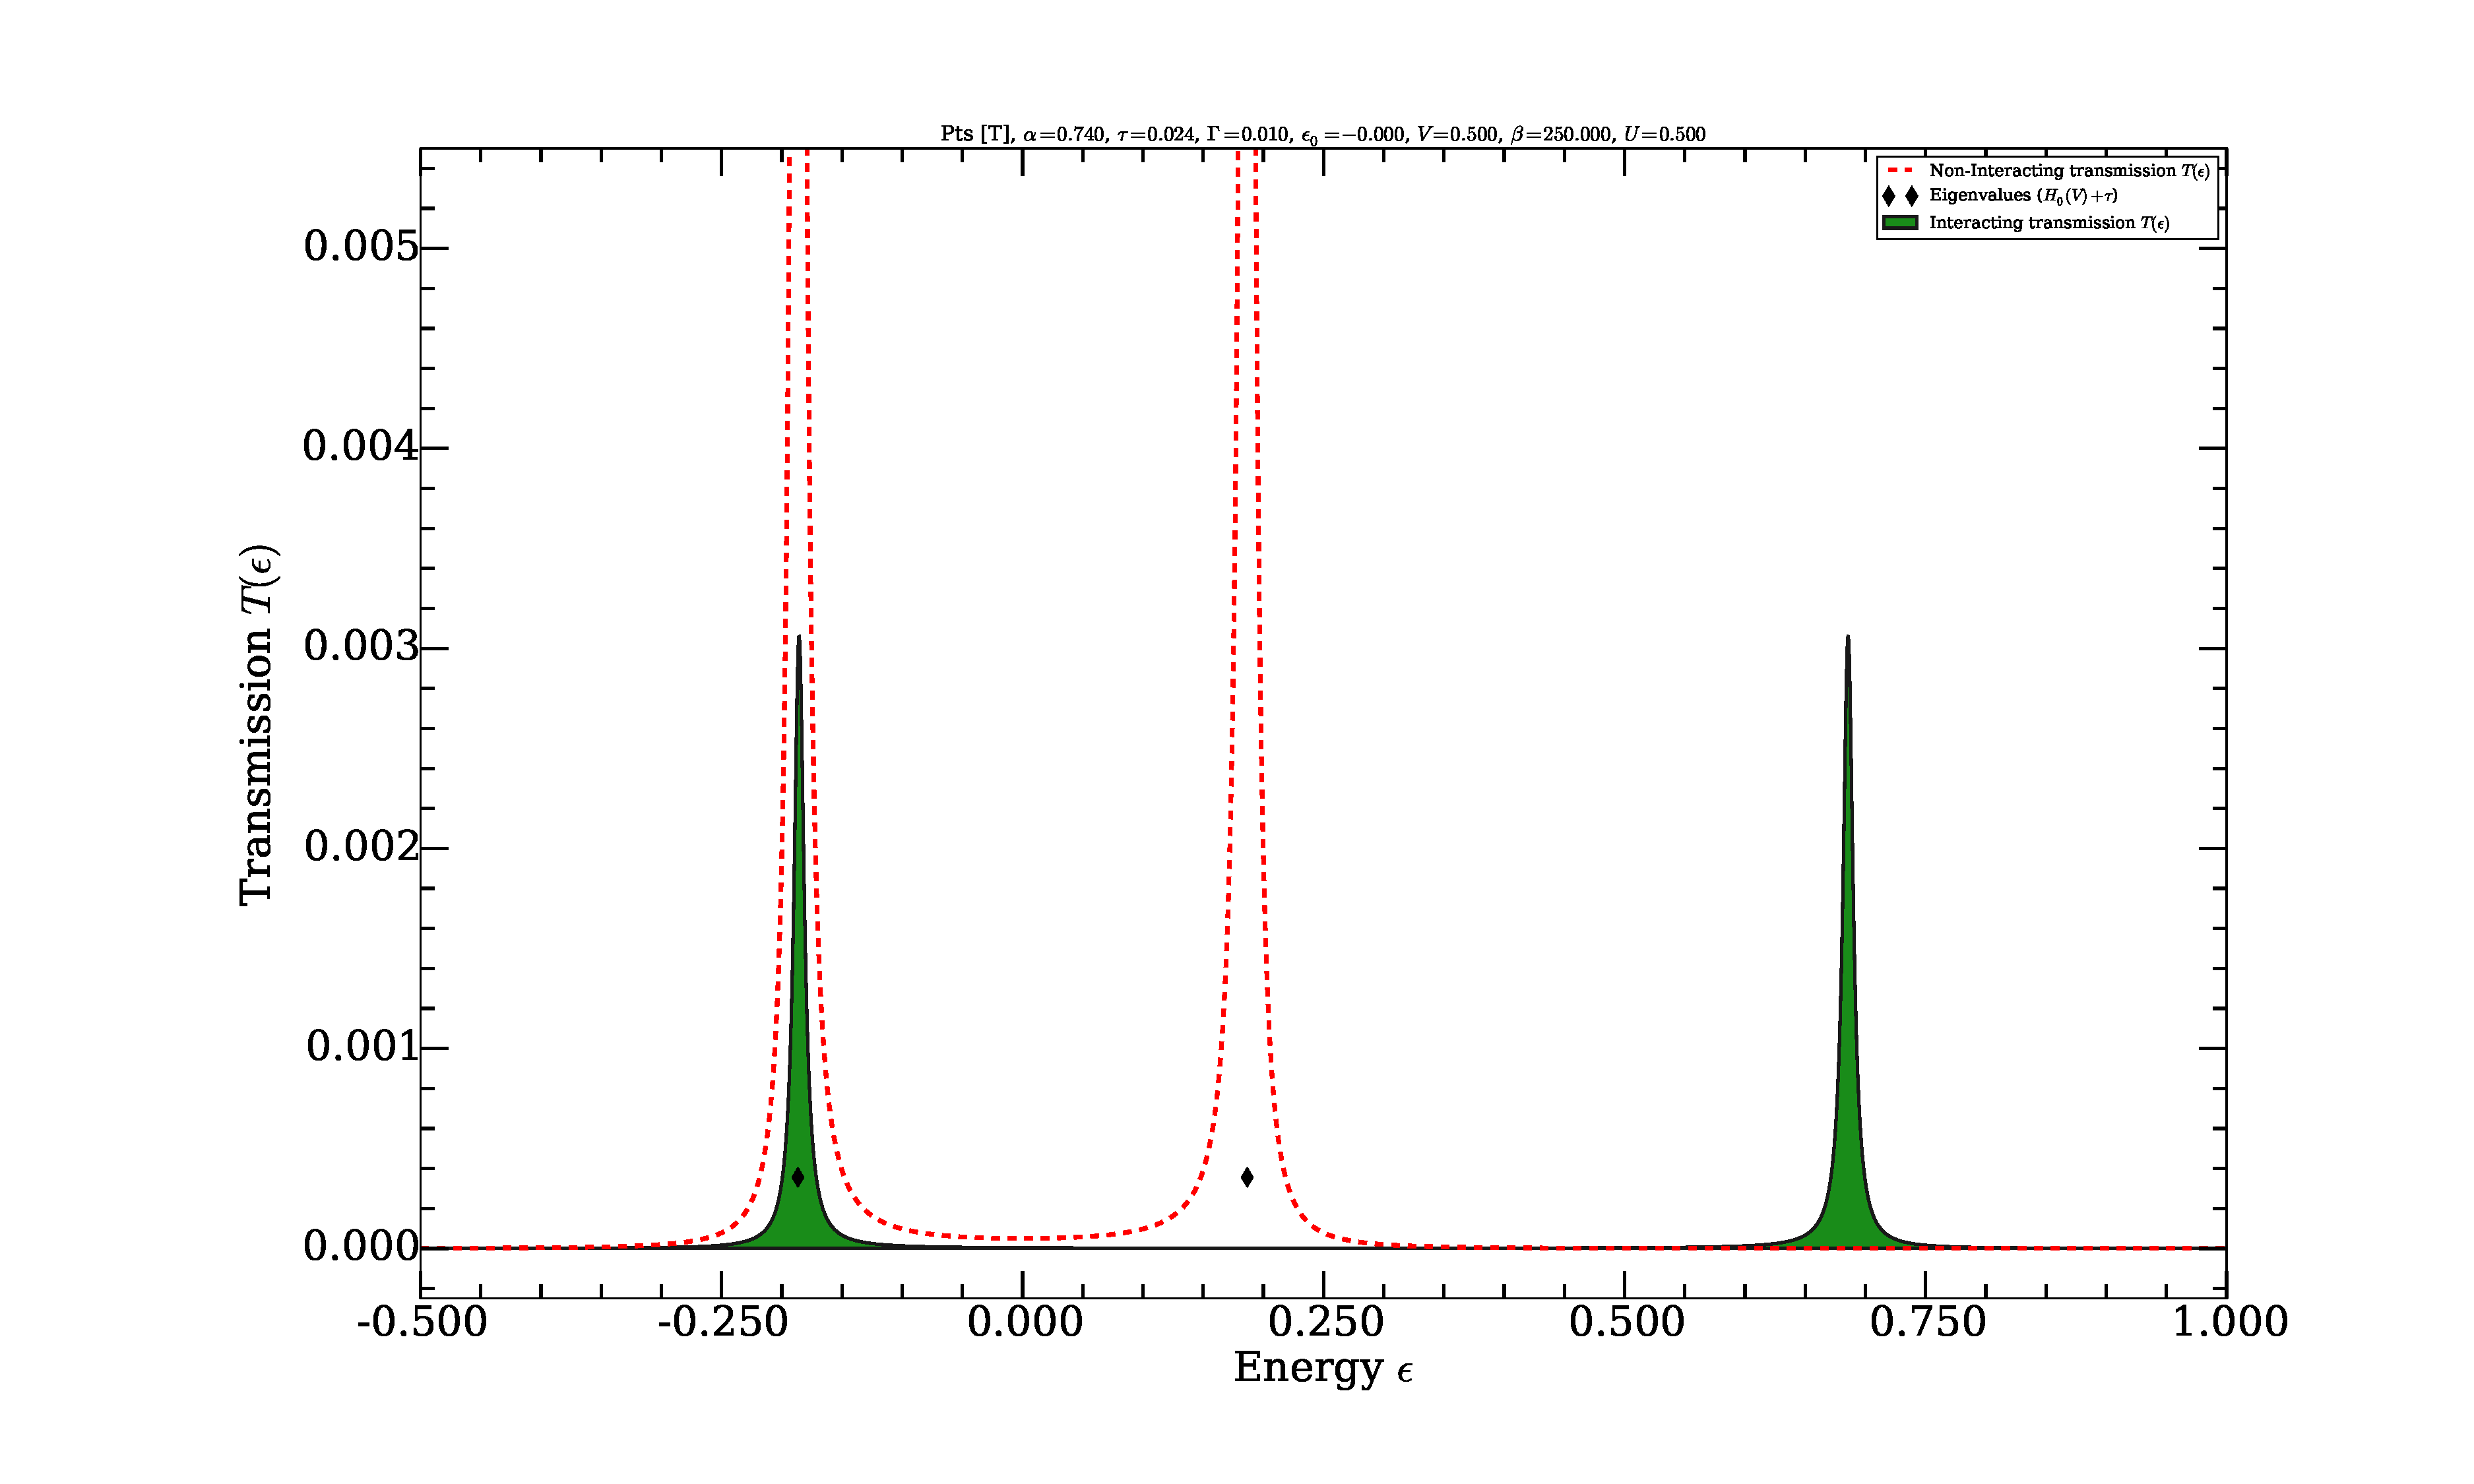
\includegraphics[height=.35\textheight,clip=true,trim=5cm 2cm 4cm 3cm]{pdf/trans/perrin_two_site.pdf}
    \caption{Non-interacting (dashed red) and interacting (green) transmission spectra for $\alpha=0.74$, $\tau=0.024$, $\Gamma=0.010$, $\epsilon_0 = 0$, $V=0.50$ and $U=0.5$. In comparison with the non-interacting transmission, the peaks have dropped significantly and the rightmost peak is exactly $U$ removed from the corresponding eigenvalue (black diamonds).}
    \label{fig:spinlesstransmission}
\end{figure}

The interacting transmission spectrum looks similar to a non-interacting transmission spectrum, but the peak values differ. It is perhaps illustrative to consider Figure~\ref{fig:perrin_effective}. In this figure the `effective parameters' change almost linearly with increasing $U$. The effective parameters are those parameters for which the features of the transmission agree with a non-interacting model ignoring peak height.
\begin{figure}[htb]
    \centering
    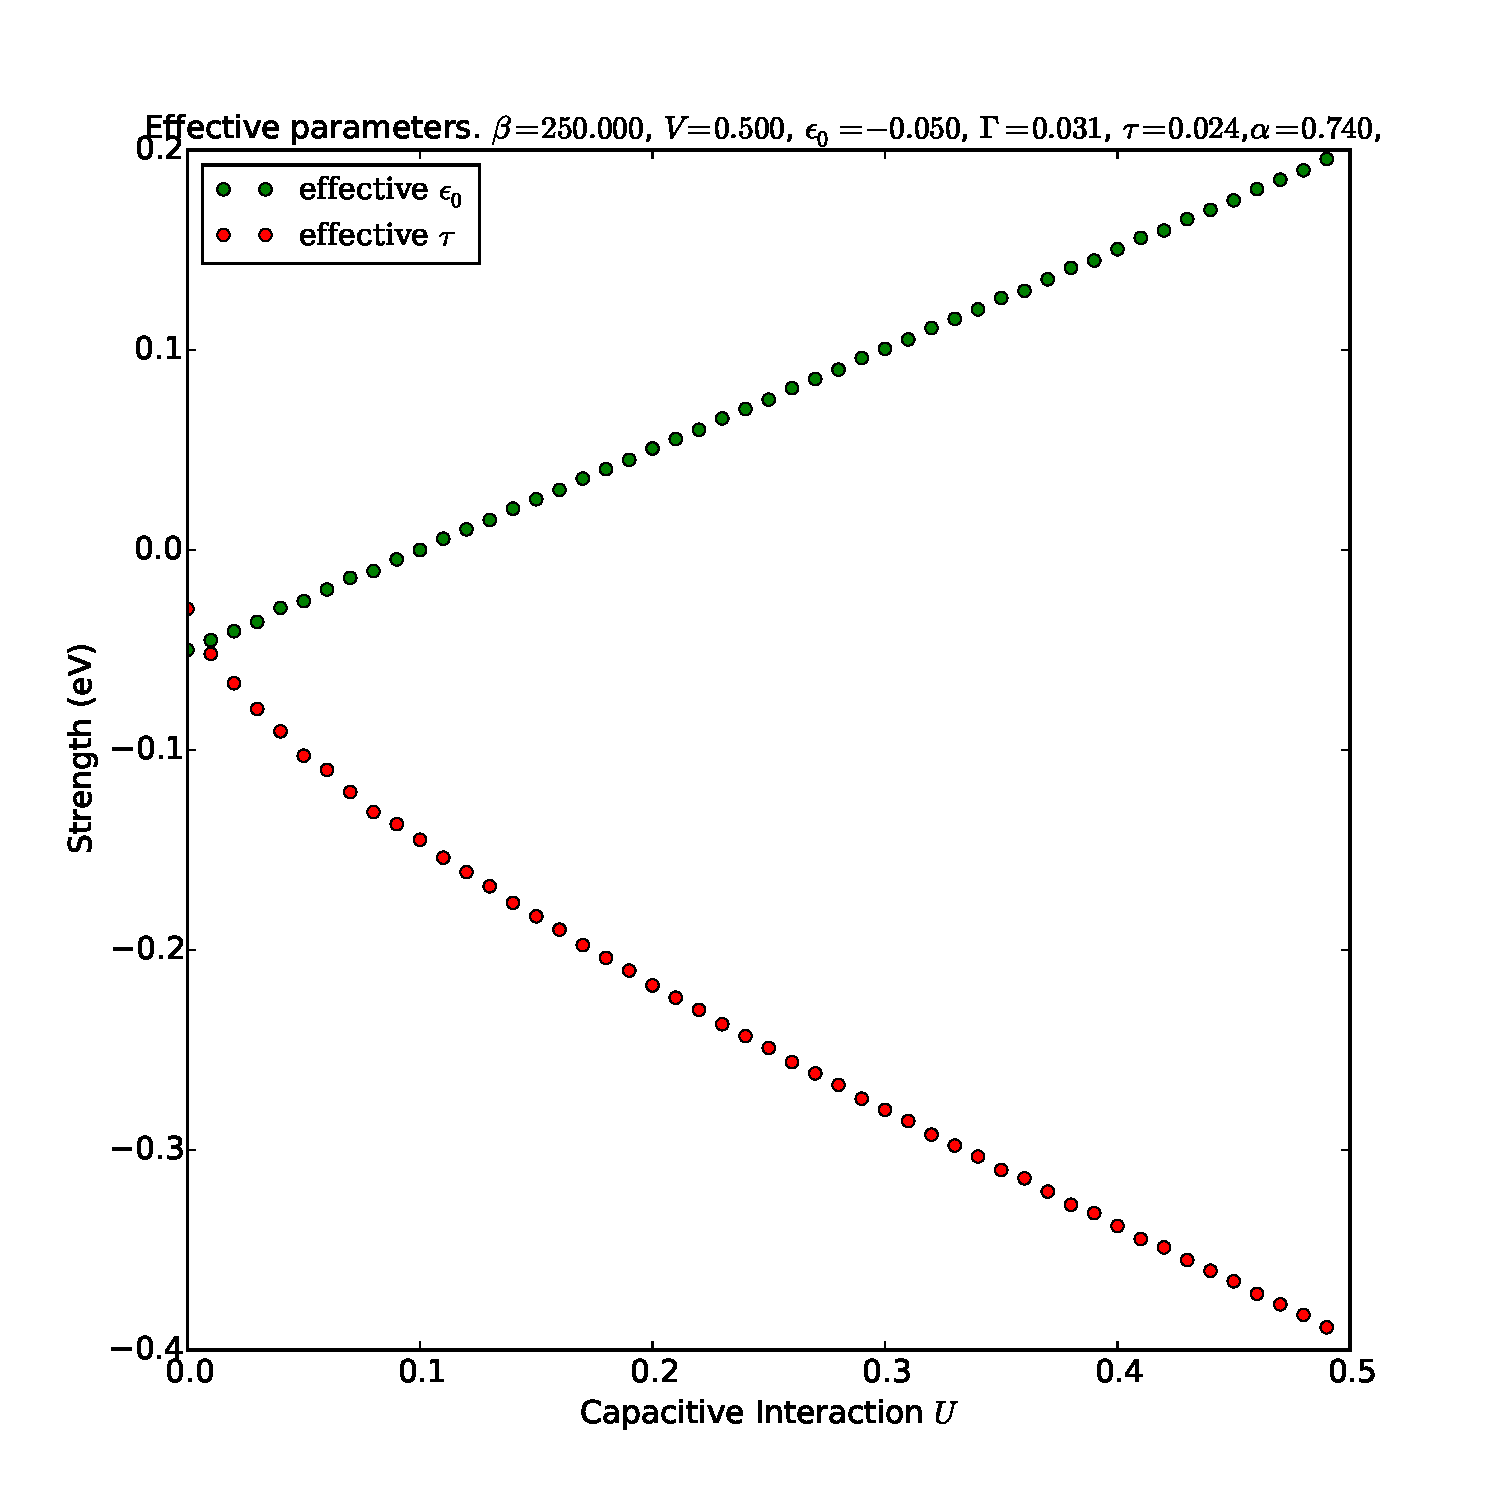
\includegraphics[height=.35\textheight]{pdf/trans/perrin_effective.pdf}
    \caption{In this figure, $\epsilon_0$ and $\tau$ are for a non-interacting model that is fitted to an interacting model, leading to `effective' parameters. This ignores the fact that the peaks of an interacting are suppressed. }
    \label{fig:perrin_effective}
\end{figure}


These figures indicate that a mismatch in peak values such as that found in Ref.~\cite{perrinnano} may well be explained in terms of capacitive interaction. Here, the shape would be fitting for a two-site model without capacitive interaction, but the amplitude element of capacitive interaction is merely seen as quantitative disagreement. This notion will be discussed further in section~\ref{sec:perrin}. 

\subsection{Spinfull two-site model}
I now want to look at the transmission of the spinfull model \emph{in comparison} with that of the spinless model. First, recall that $\zeta$ describes the intersite interaction while $\xi$ the onsite interaction. Given the large amount of possible pictures, here I present only those that are interesting results that are distinct from the spinless model with the exception of Figure~\ref{fig:transmap34} which has extremely strong onsite interaction $\xi$ such that the two models are expected to converge. 
  
\begin{figure}[htb]
    \centering
    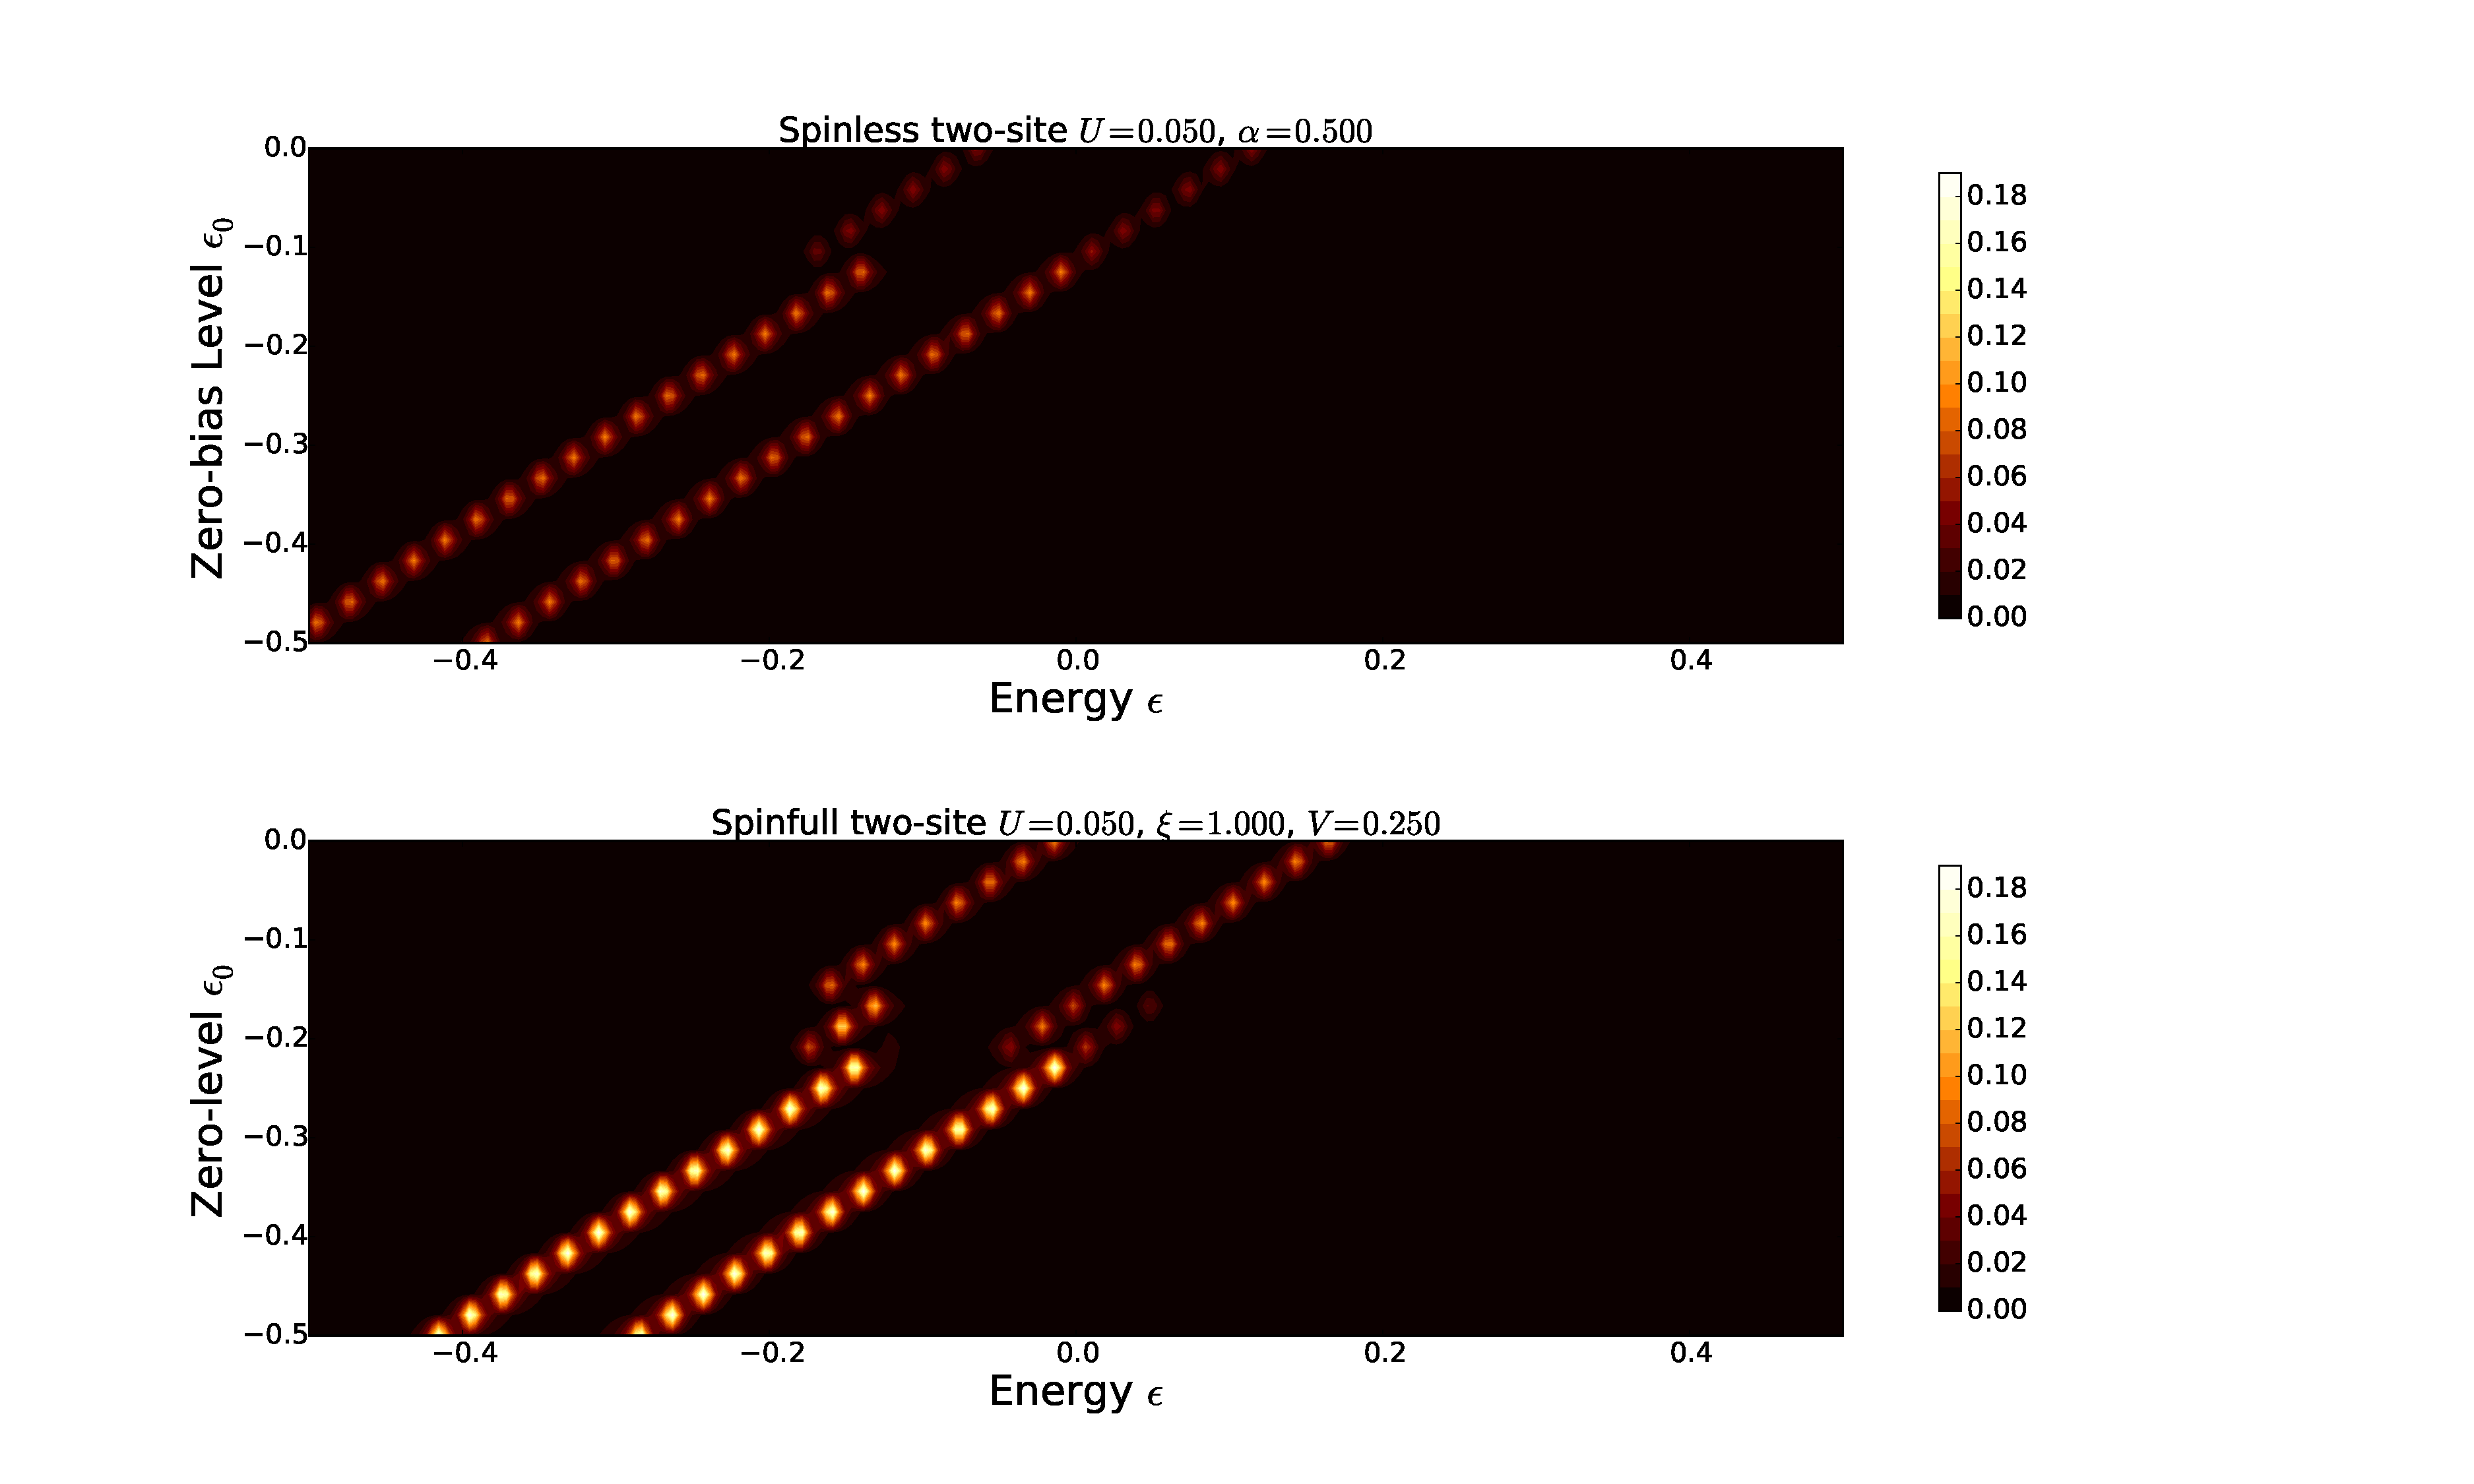
\includegraphics[height=.38\textheight]{pdf/map/transmap_u1_k2.pdf}
    \caption{In this figure, $U=0.05, \zeta=1.00, \xi=1.00$. A distinct difference is very clear, with a three-peak transmission spectrum making a short appearance. See the main text for explanation.}
    \label{fig:transmap12}
\end{figure} 
\begin{figure}[htb]
    \centering
    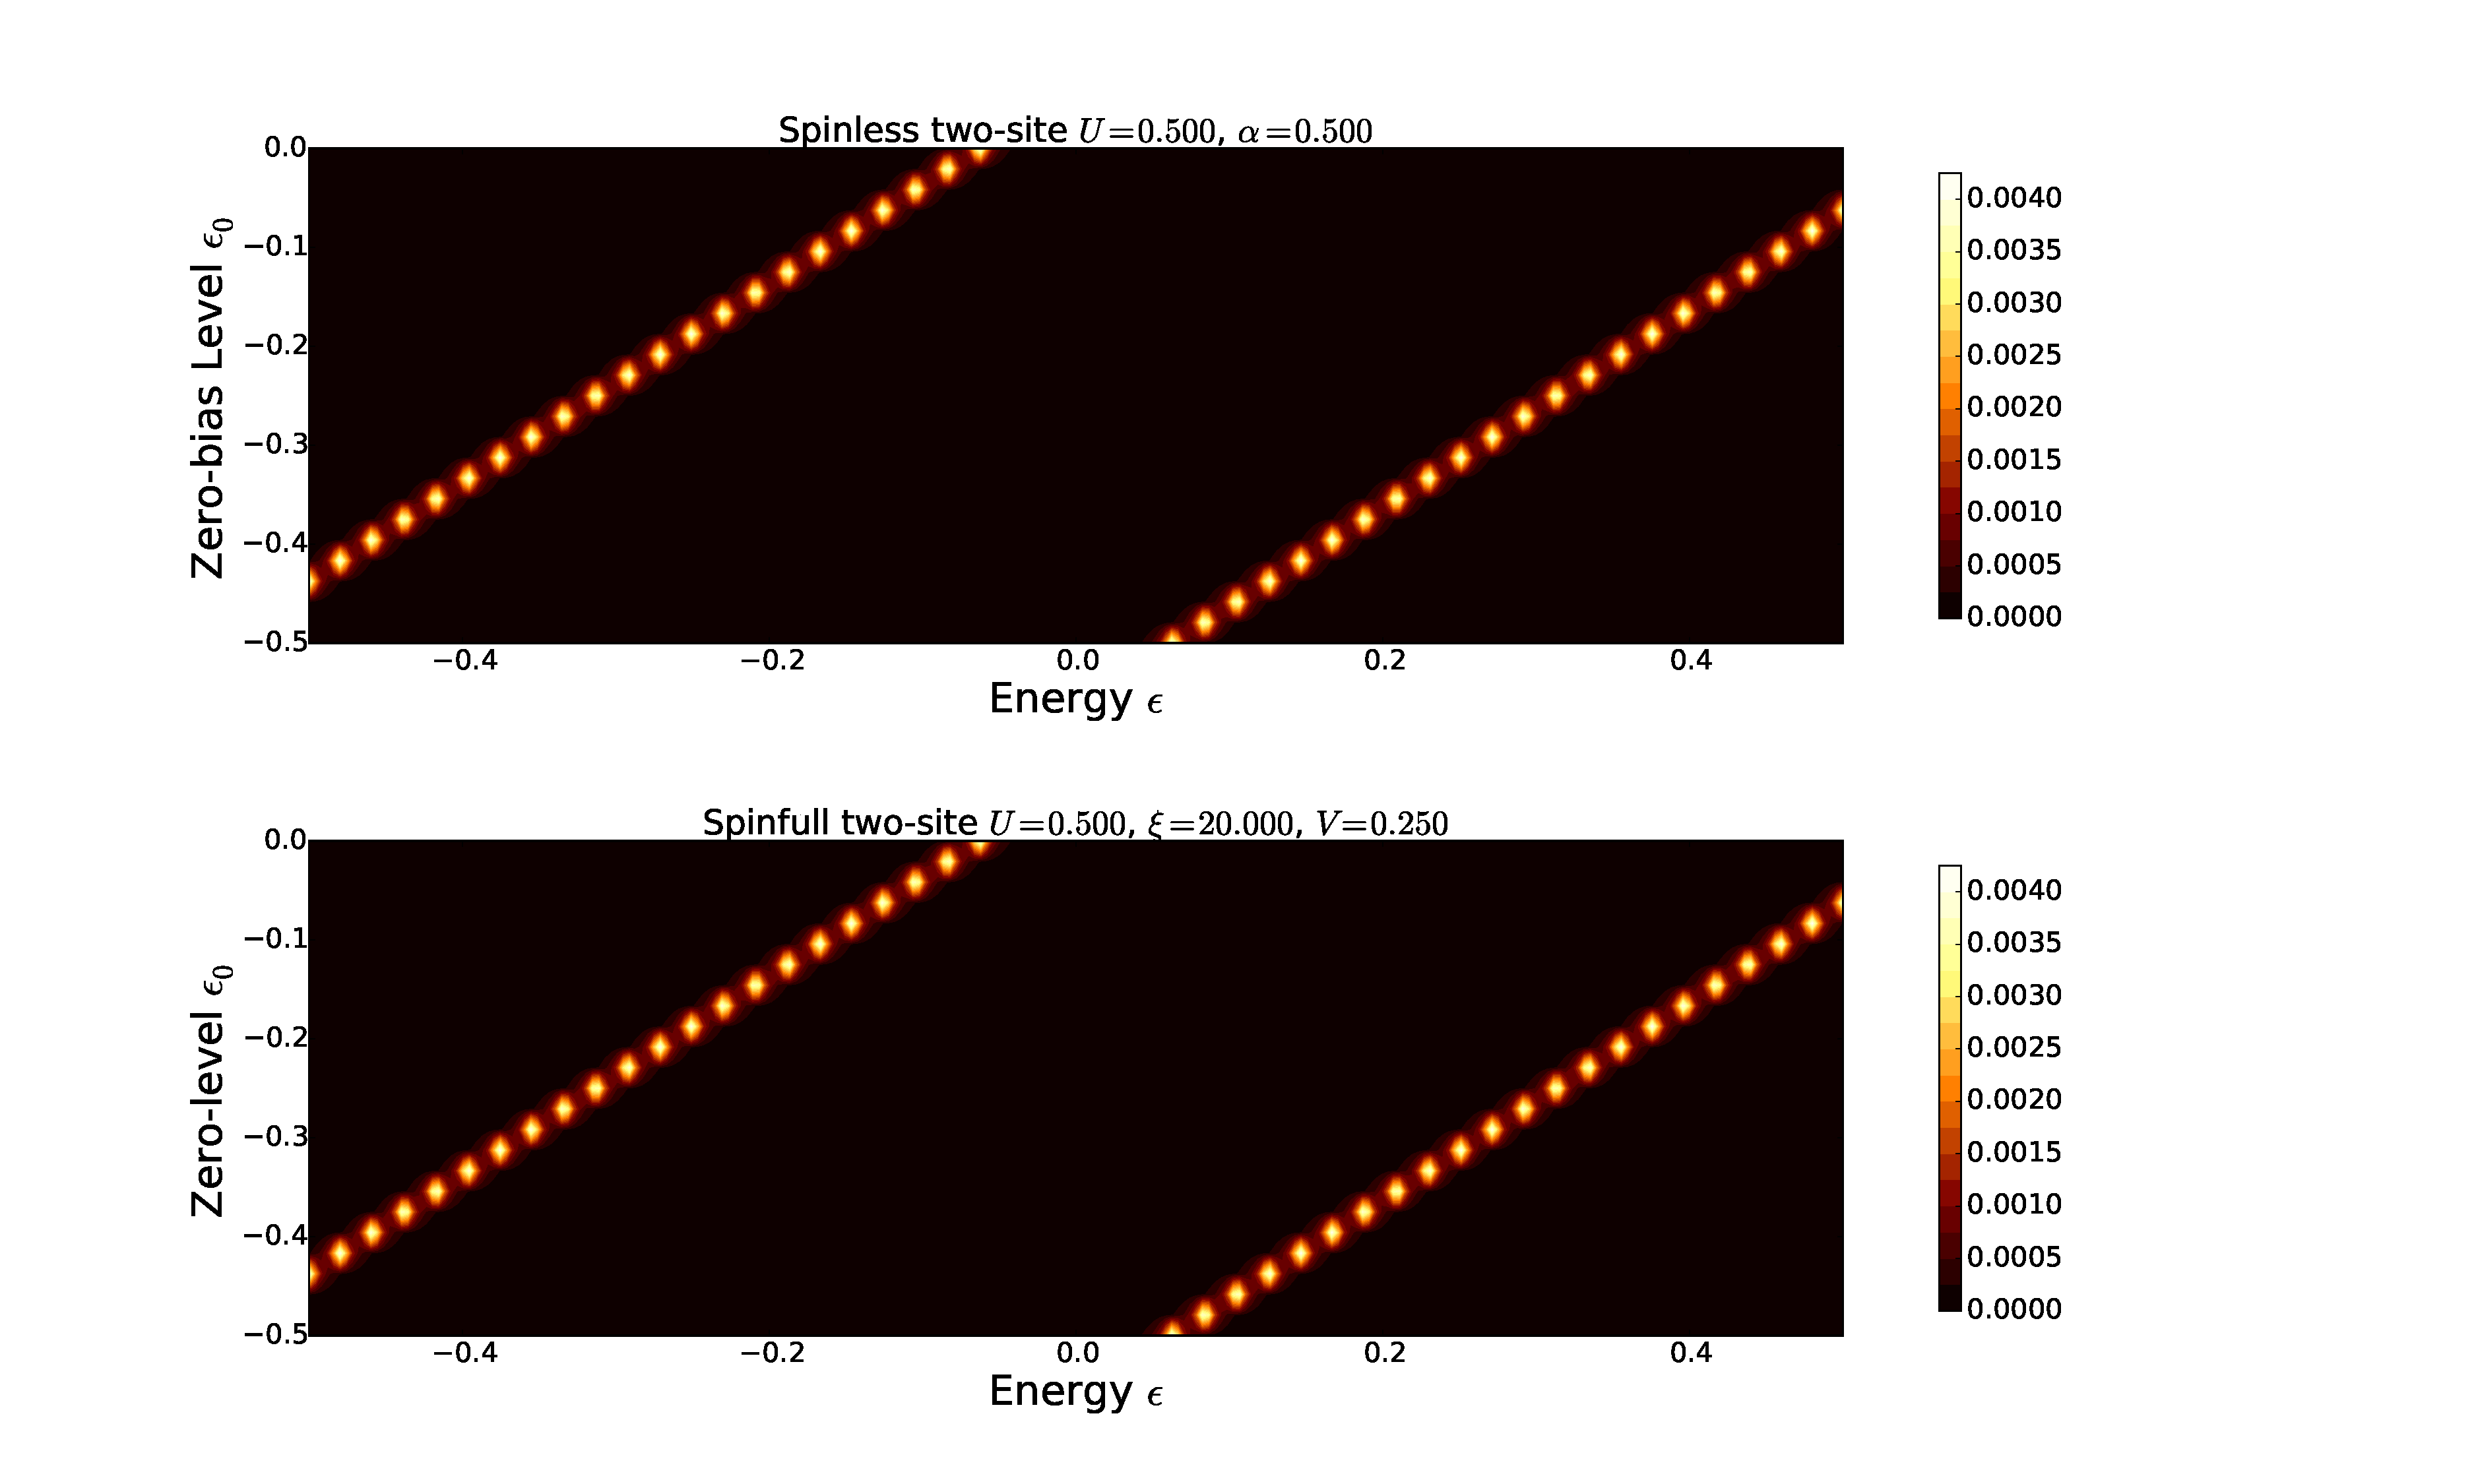
\includegraphics[height=.38\textheight]{pdf/map/transmap_u3_k4.pdf}
    \caption{In this figure, $U=0.15, \zeta=1.00, \xi=20.00$. The two models converge, which is expected for this $\xi$. See the main text for explanation.}
    \label{fig:transmap34}
\end{figure}

Evidence of the many-body character of both models is clear in Figure~\ref{fig:transmap12}, where there is one switch in transmission peaks for the spinless model and two switches for the spinfull model. The spinless model switches from $\ket{01}$ to $\ket{11}$ (Figure~\ref{fig:perrinenergy1}), displacing one peak by an amount $U$ which agrees well with the transmission figure.  The spinfull model, on the other hand, switches from $\ket{0011}$ to either $\ket{0111}$ or $\ket{1011}$ before switching to $\ket{1111}$ (Figure~\ref{fig:perspinenergy12}). Note that the rightmost peaks corresponds to the left site, and the leftmost peak corresponds to the right site. The first switch displaces the leftmost peak\footnote{Adding an electron to the left level adds $U$ to the right level, which displaces the left peak.}and seems to have placed a third peak at the rightmost peak plus $U$, a likely result because the energy states are degenerate. The second switch then displaces the leftmost peak by $\xi U$. 
 
Figure~\ref{fig:transmap34} is that figure for which the onsite energy $\xi U$ dominates so that only a single copy of the spinless model is active at any time. Therefore, not only do the peaks in transmission happen at the same location, but they are also of the same height.
\section{Current parameter sweeps}
\label{sec:twositeparamsweep}
The most interesting parameter sweeps are those that affect the many-body states. The current through a single-molecule has a well known feature called the Coulomb Diamond \cite{seldenthuis, perrin} in a plot of the gate voltage versus the bias voltage and coloured by the current. The gate voltage corresponds approximately to the zero-bias level, $V_\text{gate} \approx \epsilon_0$. Each diamond corresponds to a different charge state. As I only present current parameter sweeps for the spinless case, for which throughout $-0.5 < \epsilon_0 < 0$ there are two occupied many-body states, we expect one diamond to form.  

\begin{figure}[htb]
    \centering
    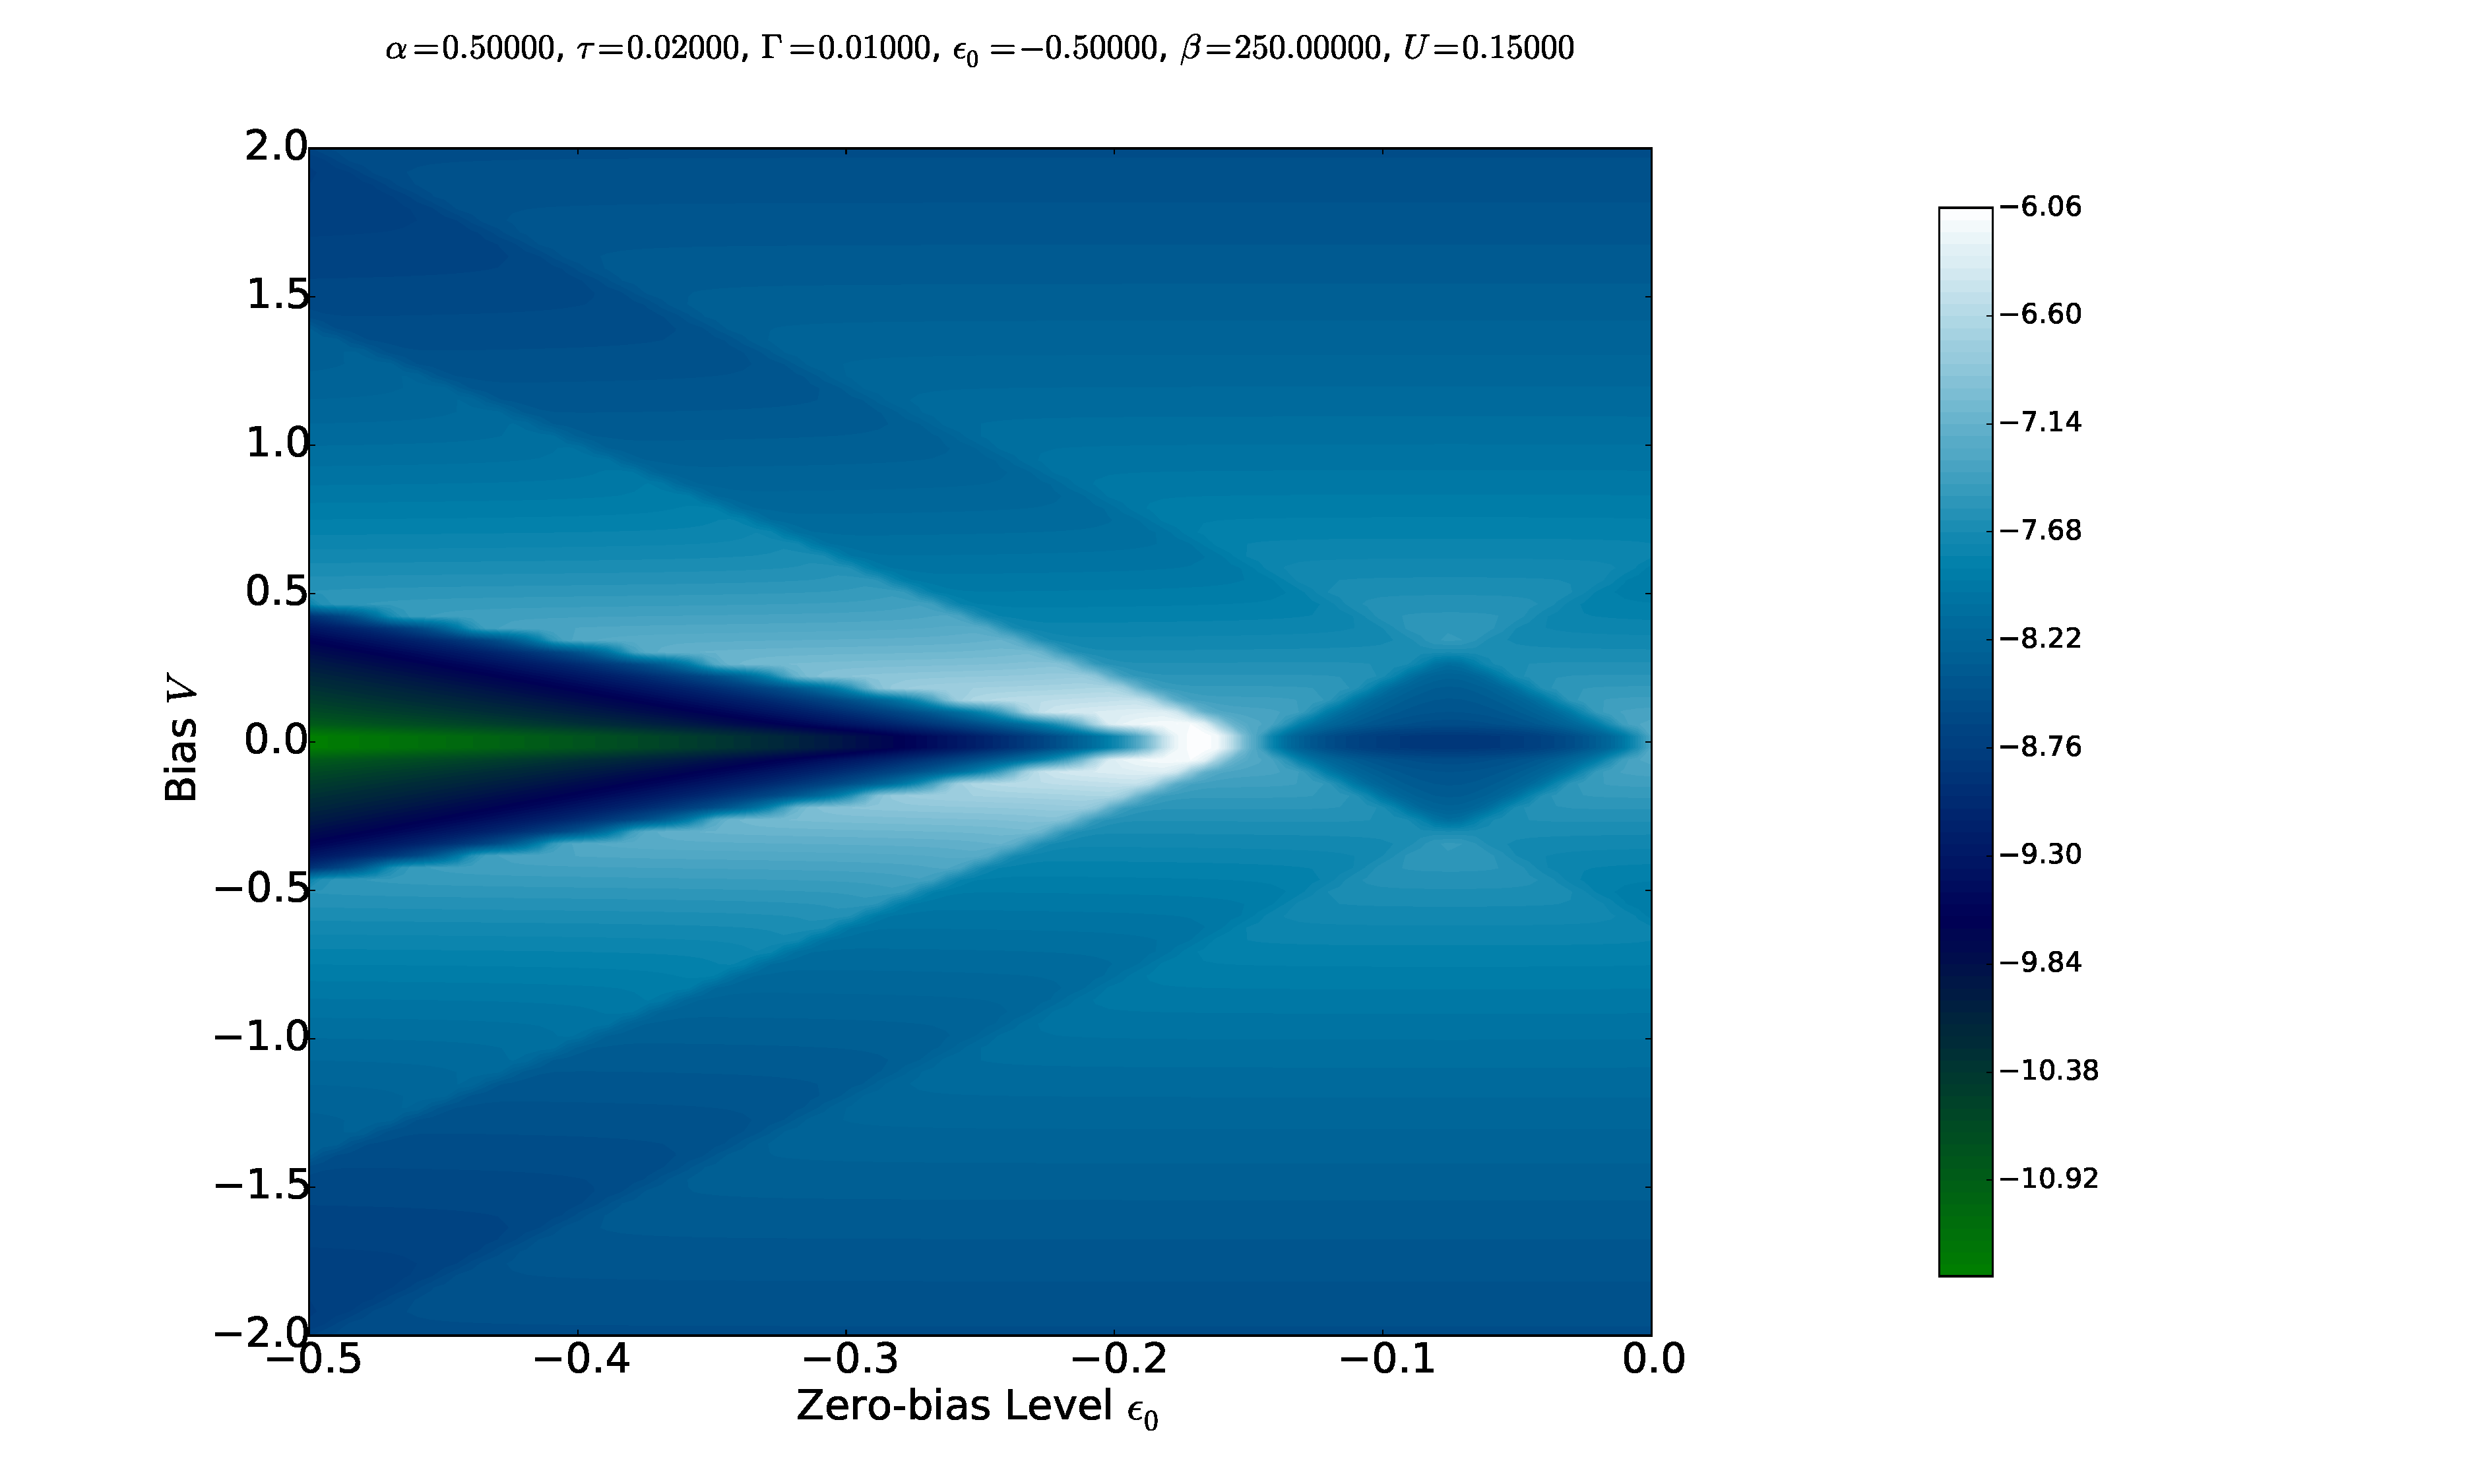
\includegraphics[height=.38\textheight]{pdf/coulombd/current_map_u2.pdf}
    \caption{In this figure, $U=0.15$. The Coulomb diamond is singificantly clearer and again has width $U$. The triangular area to the left of the diamond corresponds to the next charge state. The distinct lines correspond to the bias window increasing to encompass a second transmission peak.The colours are based on the $^{10}\text{log}\left|I(V)\right|$, so that the NDC is implied because $I(V) = -I(-V)$.}
    \label{fig:currentmap2}
\end{figure} 

Figures~\ref{fig:currentmap2} and ~\ref{fig:diamond50} show the onset of the Coulomb diamond and that its width exactly equals the capacitive interaction strength $U$. The left triangular area visible in most of the figures is the next charge state, which for the spinless model is the state $\ket{11}$ whereas the Coulomb diamond is associated with $\ket{01}$ (at positive bias). 

I explored the characteristics of the Coulomb Diamond a bit more. Analytically, the corresponding charge state leads to the following Green's function (section~\ref{sec:twosite}):
\begin{align*}
G^{\ket{01}\pm} &= \left[ \epsilon \begin{bmatrix} 1 & 0 \\ 0 & 1 \end{bmatrix} - \begin{bmatrix} \epsilon_0 + \frac{1}{2} \alpha V & -\tau \\
-\tau & \epsilon_0 - \frac{1}{2} \alpha V\end{bmatrix} - \begin{pmatrix} U & 0 \\ 0 & 0 \end{pmatrix} \pm \frac{\imath}{2} \begin{pmatrix} \Gamma & 0 \\ 0 & \Gamma \end{pmatrix} \right]^{-1},
\end{align*}
so that the transmission peaks should be found at eigenvalues of $\begin{bmatrix} \epsilon_0 + \frac{1}{2} \alpha V+U & -\tau \\
-\tau & \epsilon_0 - \frac{1}{2} \alpha V\end{bmatrix}$.

Section~\ref{sec:twositetransmission} showed that the transmission peak locations change linearly with $\epsilon_0$, at least within a single charge state. Consider a state which starts on resonance, i.e. a transmission peak is within the bias window immediately. In this scenario, the leftmost transmission peak is within the bias window. Upon lowering $\epsilon_0$, the two transmission peaks shift slightly to the left. At higher bias, the intersection of the leftmost peak with the bias window is still at a lower bias voltage than that of the rightmost peak, but at a larger bias voltage than at higher $\epsilon_0$. As the lowering continues, the two values slowly approach each other. This is the corner of the Coulomb diamond.

Next, the the rightmost peak has the lower bias voltage at which it intersects the bias window and this intersection value is shrinking. This continues until the point where the rightmost peak is completely inside the bias window. This closes the diamond. 

The expectation is that the next charge state is then available, and indeed I find that the energies dictate the molecule now occupies the next charge state.

The rate at which the transmission lines move outward depends almost entirely on $\alpha$. While it is technically the level-splitting $\Delta$, it is trivial that as the only growing term it will soon dominate that term, leading to $\Delta \approx \alpha V$. As such, I expect that the height of the Coulomb diamond depends mostly on $\alpha$. 

Indeed, this is what we find Figures~\ref{fig:diamond50} and ~\ref{fig:diamond75}. These figures also show the co-tunneling current within the diamond clearly. Here, the symmetry dictates that $I(V)=-I(-V)$, so that the co-tunneling current has a sign switch around $V=0$. Furthermore, the Stark effect pulls the sites further from each other, which leads to a reduction of the co-tunnelling current that is just barely visible. 
\begin{figure}[htb]
    \centering
    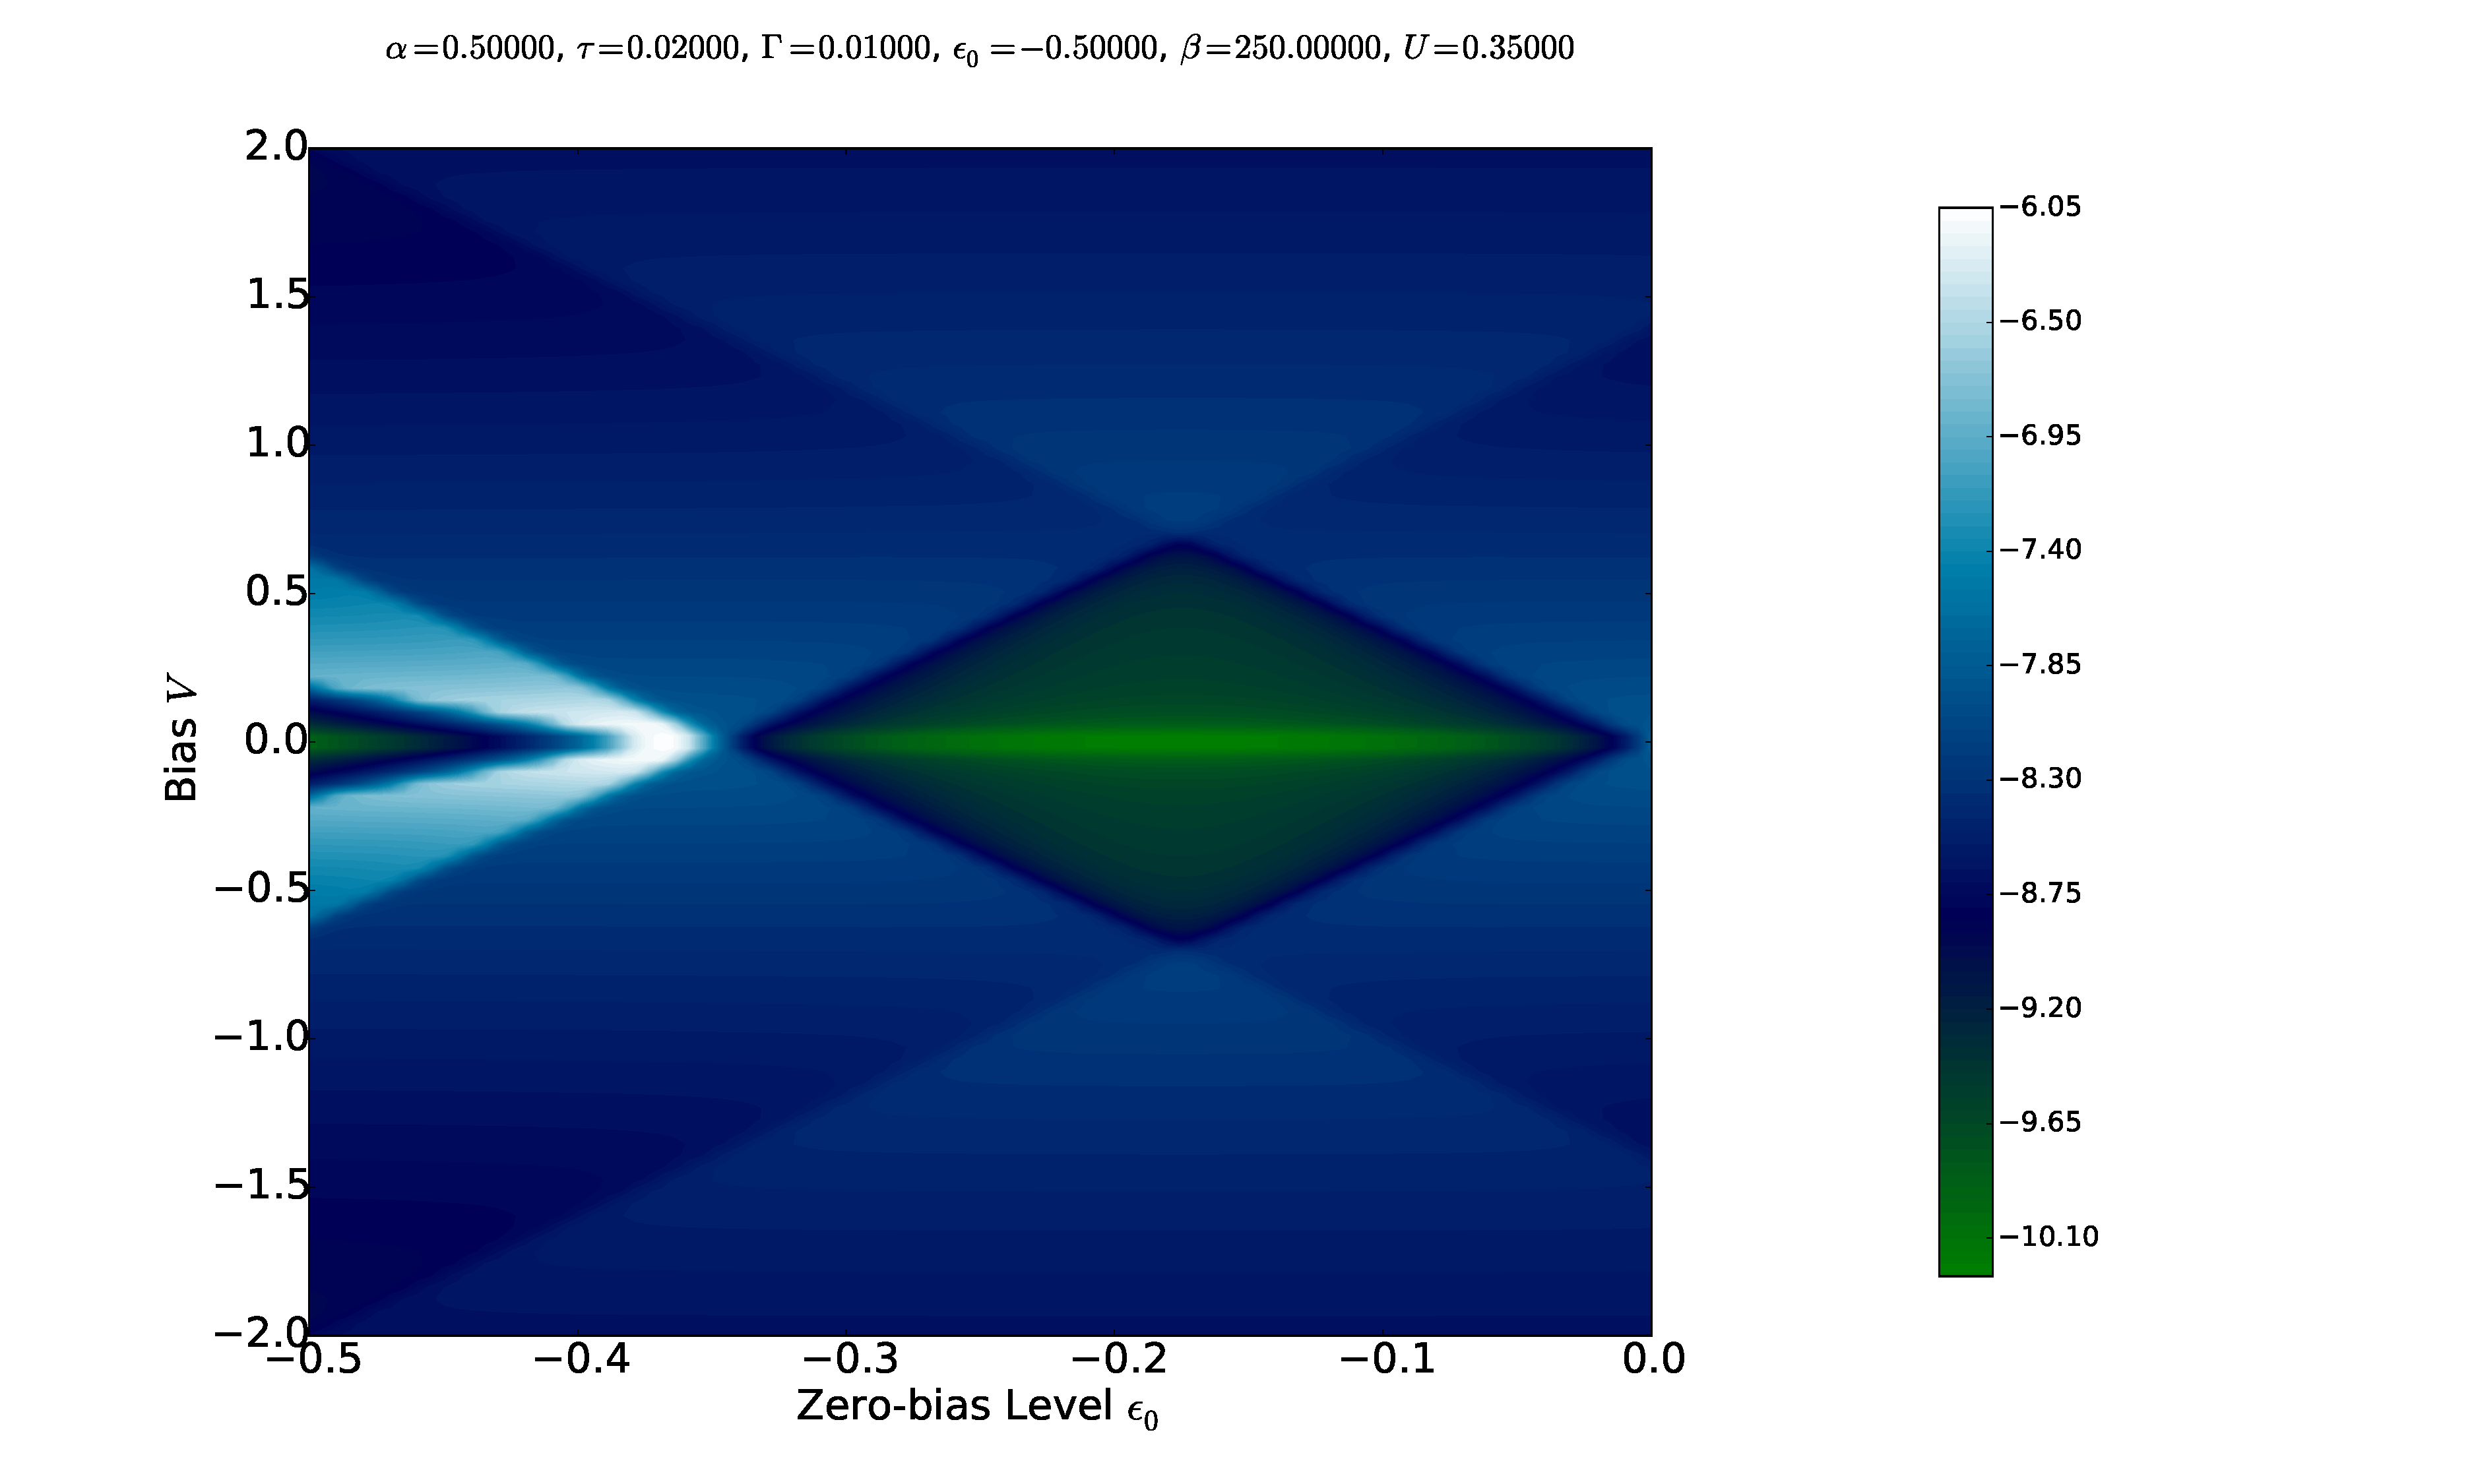
\includegraphics[height=.38\textheight]{pdf/coulombd/current_map_diamond_alpha_05.pdf}
    \caption{In this figure, $U=0.35$ and $\alpha=0.50$. The colours are based on the $^{10}\text{log}\left|I(V)\right|$, so that the NDC is implied because $I(V) = -I(-V)$.}
    \label{fig:diamond50}
\end{figure}
\begin{figure}[htb]
    \centering
    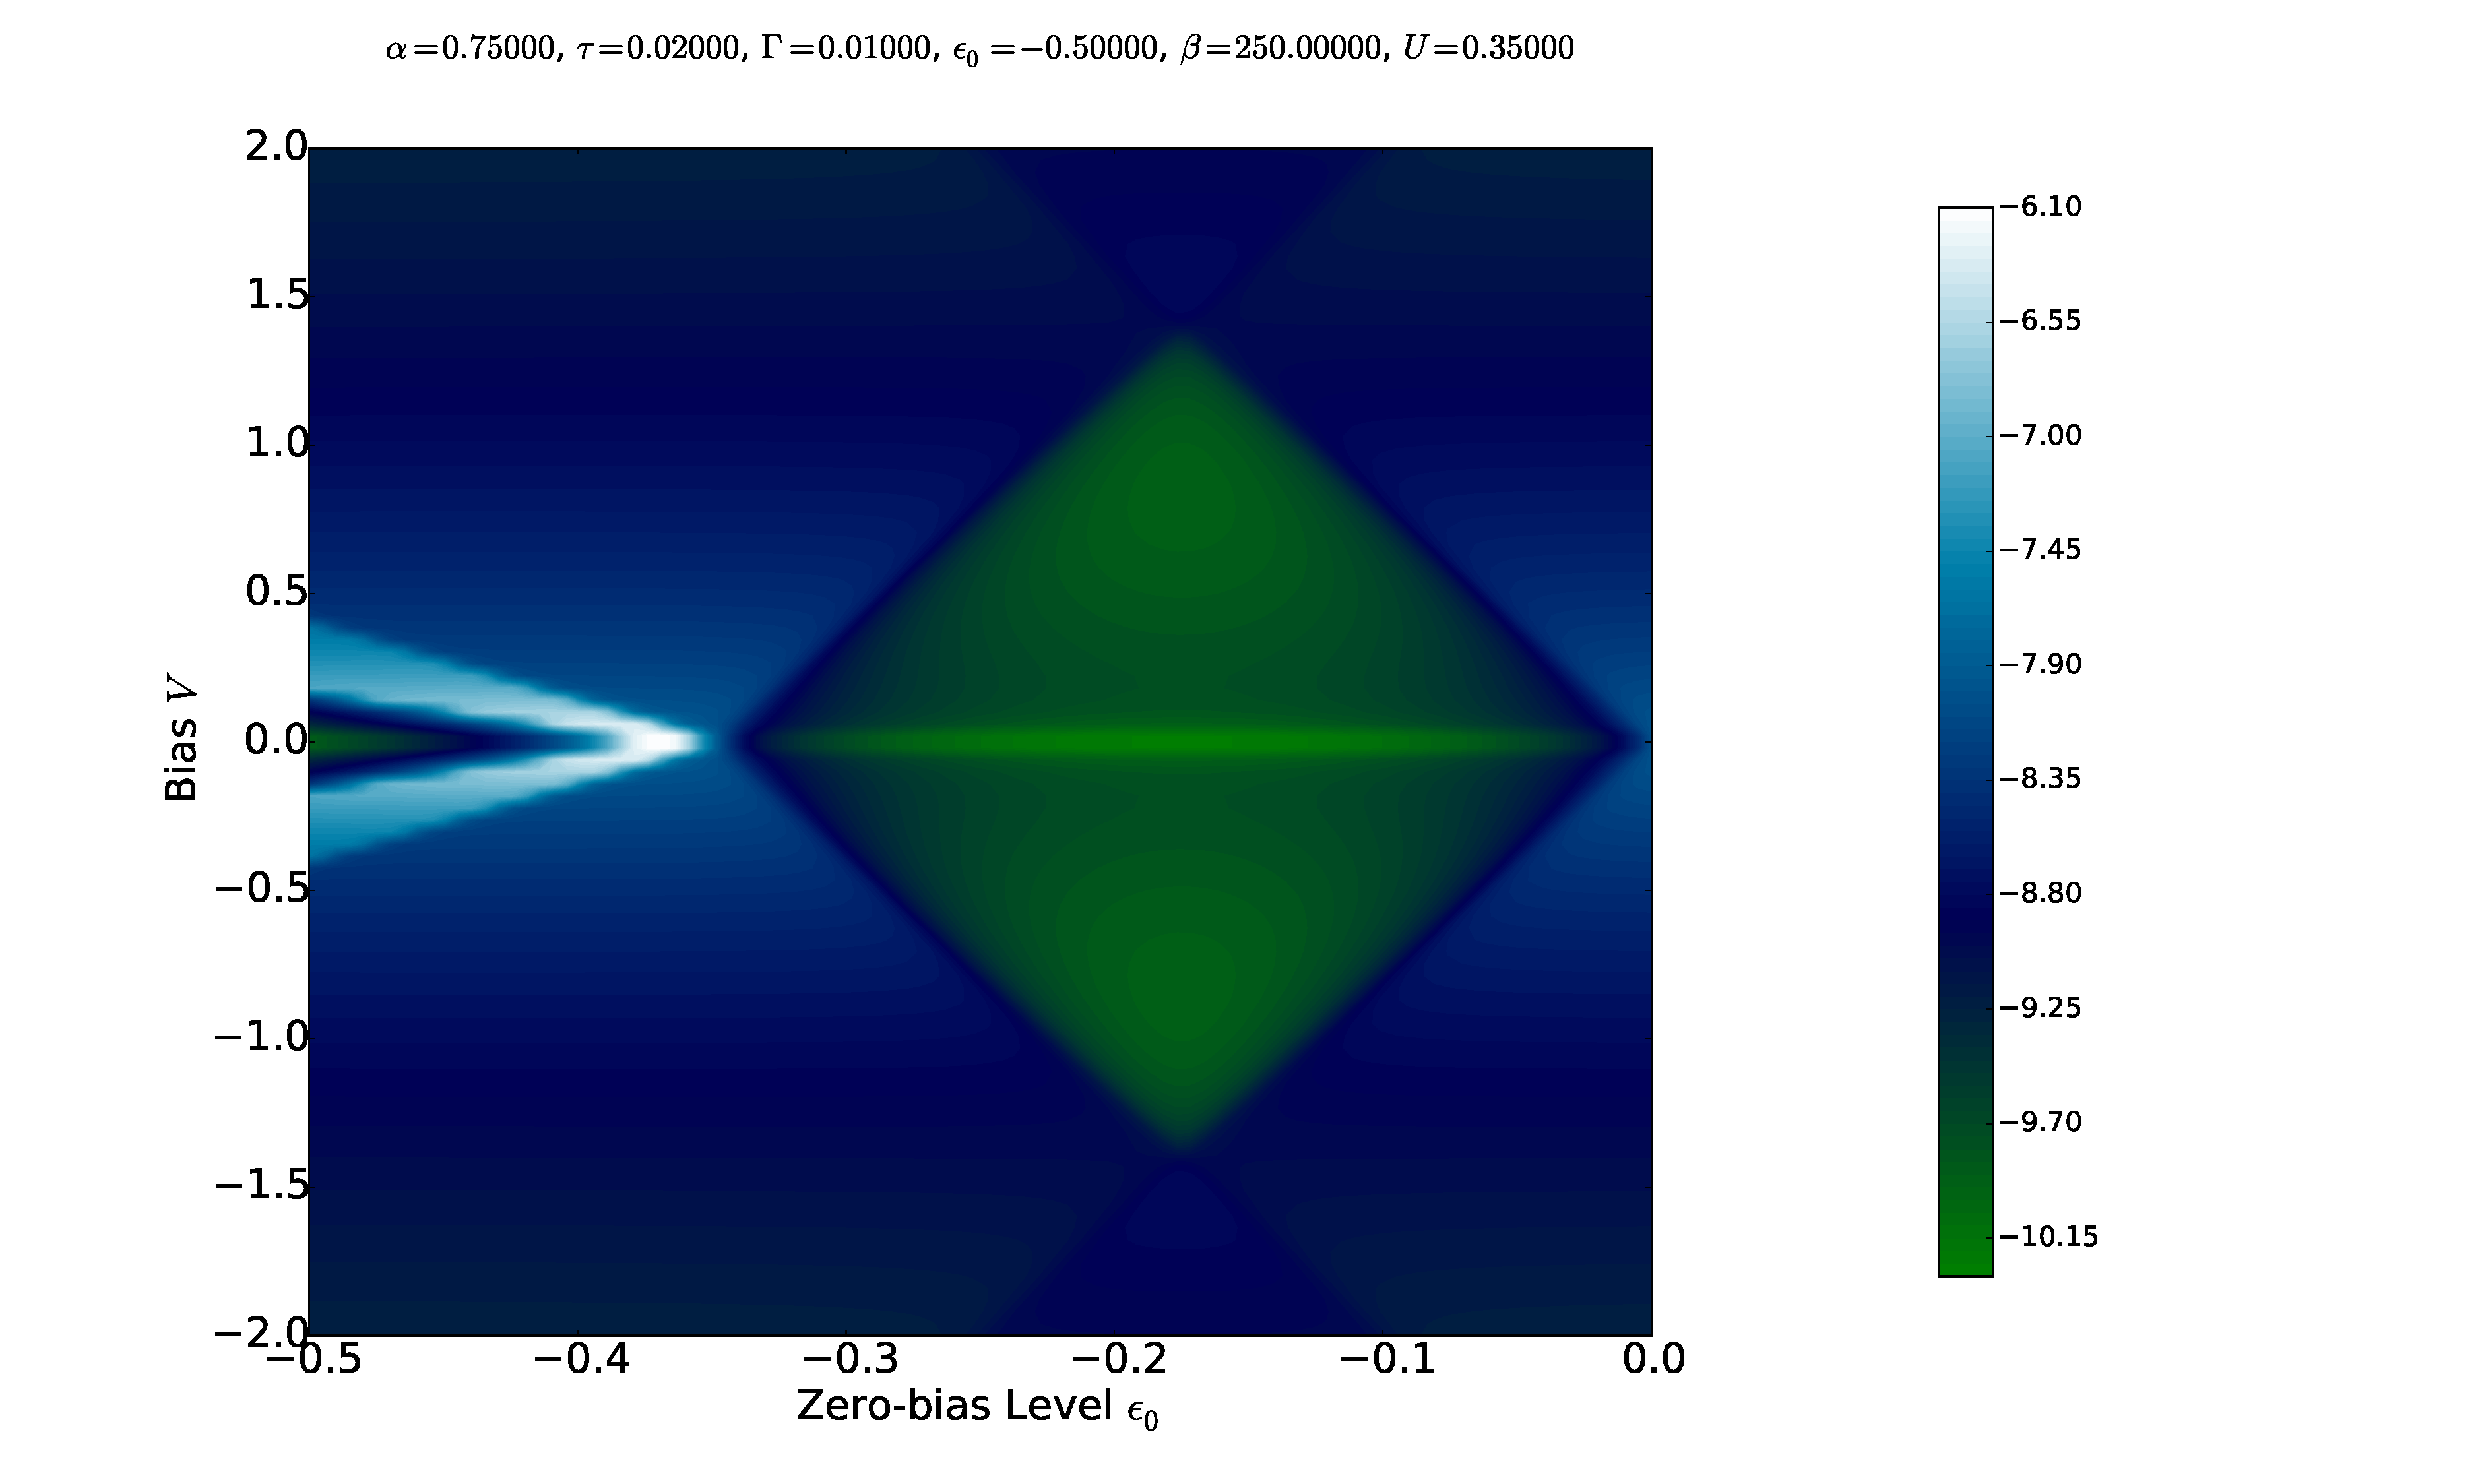
\includegraphics[height=.38\textheight]{pdf/coulombd/current_map_diamond_alpha_075.pdf}
    \caption{In this figure, $U=0.35$ and $\alpha=0.75$. The colours are based on the $^{10}\text{log}\left|I(V)\right|$, so that the NDC is implied because $I(V) = -I(-V)$.}
    \label{fig:diamond75}
\end{figure}

\section{Experimental fit}
\label{sec:perrin}
On inspection of the peak values of current when the many-body occupation is the first charge state, I found that the current was already less than it was in \citet{perrinnano} or the zero-charge state. In Figure~\ref{fig:imax}, I compare the peak current at certain capacitive interaction strength for the edge of the first and second charge states. The first charge state has the left and right sites at different energies, so that current is suppressed relative to the second charge state which has both levels at the same energy.
\begin{figure}[htb]
    \centering
    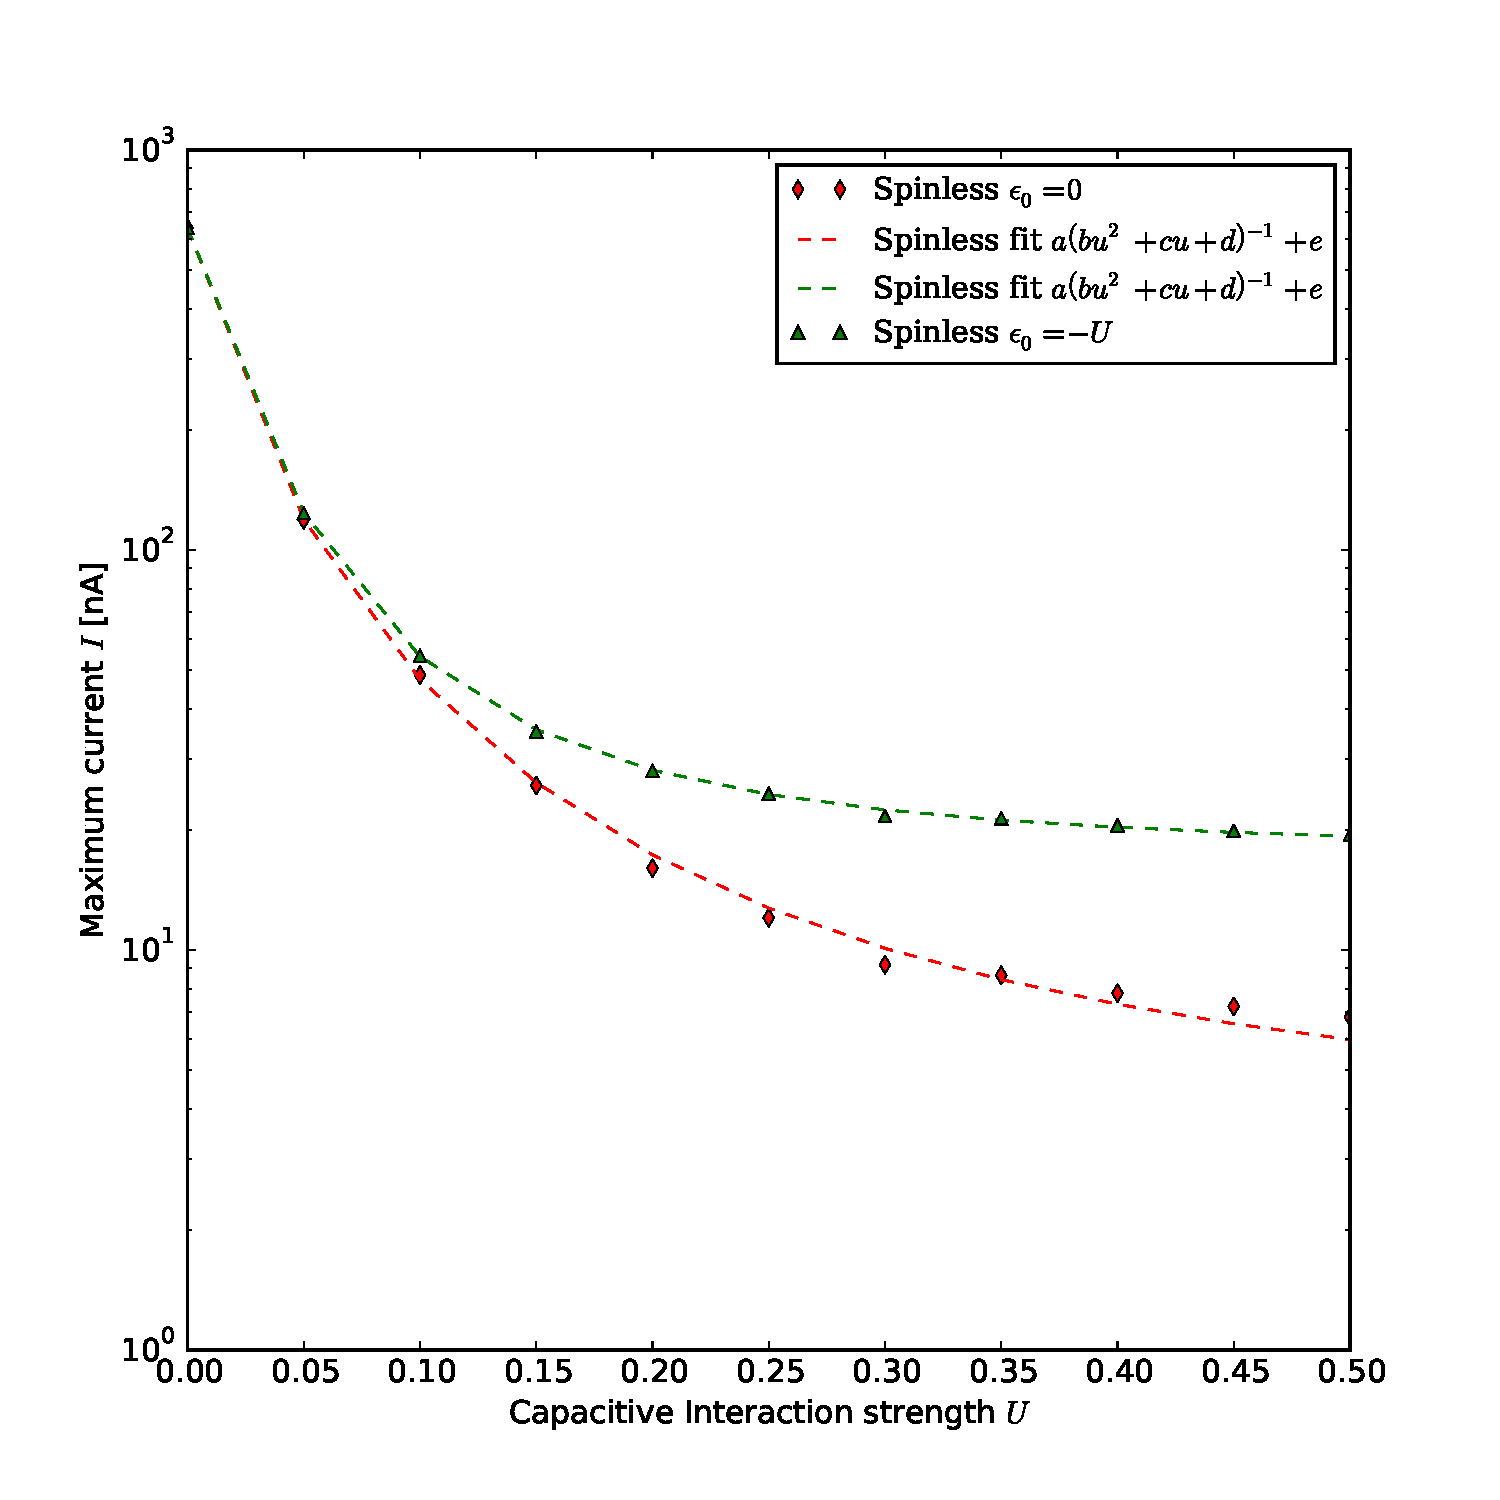
\includegraphics[height=.38\textheight]{pdf/imax.pdf}
    \caption{In this figure, $\alpha=0.50$, $\tau=0.02$, $\Gamma=0.01$, $\epsilon_0 = 0$ or $\epsilon_0=-U$. I show the maximum current versus the capacitive interaction, for the first charge state (red diamonds) and the second charge state (green triangles). Visible is that the second charge state has a current that is within one order of magnitude larger, likely because the left/right levels align. Both sets fit well to a fit to an inverse polynomial of $U$. See main text for explanation.}
    \label{fig:imax}
\end{figure}

Figure~\ref{fig:imax} seems to indicate that the maximum current will flatten out, so that peak currents of approximately $10$ nA in the first charge state and approximately $5$ nA are expected for strong interaction $U \gtrsim 0.30$. This can be understood from the following. In the supplement to Ref.~\cite{perrinnano}, they compute the current for a two-site model in terms of the bonding ($\pi$) and anti-bonding ($\pi$) orbitals. The current is proportional to the inverse of the level splitting, $\left( \Delta^2 + \Gamma^2 \right)$. The level splitting for the interacting case can be found from the eigenvalues of e.g. $\begin{bmatrix} \epsilon_0 + \frac{1}{2} \alpha V+U & -\tau \\
-\tau & \epsilon_0 - \frac{1}{2} \alpha V\end{bmatrix}$:
\begin{align*}
\Delta^2 &= U^2 + U \left(4\epsilon_0 - 2 \alpha V\right) + \alpha^2 V^2 - 4 \tau^2,
\end{align*}
so that the maximum current is proportional to the inverse of a second-order polynomial of $U$. The fits in Figure~\ref{fig:imax} show that this simply analysis yields the correct results. The second charge state is expected to yield a higher current, as $\Delta$ reduces by $4 \left|\epsilon_0 \right| U$. This agrees with the concept that the first charge state has misaligned levels, because that indicates a larger $\Delta$ and thus a lower current, whereas thee second charge state has a small $\Delta$ and a high current. However, I must caution that this analysis and Figure~\ref{fig:imax} concern only non-degenerate states.

These results indicate that the Coulomb interaction energy is in principle able to tune the peak current. Note that the Coulomb interaction energy will at some point induce a switch to a different many-body state (section~\ref{sec:expectations}). I will look at the measurements by Mickael Perrin \cite{perrin, perrinnano}, whom has kindly given me one of his datasets to look at. 

In figure~\ref{fig:perrindata}, a break junction measurement for different separation differences (gap sizes) is shown. As the separation distance increases, the current drops increasingly, until an apparent Coulomb gap opens suddenly around separation $s \approx 663$. As I showed in section~\ref{sec:expectations}, very sudden transmission changes can occur due to many-body state switches. I surmise a similar thing has happened here. As separation distance increases, we see that the $V=0$ flattish area starts increasing. At approximately $s\approx 663$, it suddenly widens and a rather clear Coulomb blockade is visible. While there is no good way to estimate the theoretical parameters from such an experiment, speculation is possible. If all parameters change slowly, then this could simultaneously explain both the peak current dropping and the opening of a flat area in between. For $s \lesssim 663$, the zero charge state is likely occupied, based on the current at $s = 638$ and the smooth change from there. The zero bias level $\epsilon_0$ slowly move off-resonance as separation increases, which is the opening of the plateau. Then, at $s \approx 663$, a many-body switch happens and the molecule is found in the first charge state. As $\epsilon_0 \neq 0 $ and $\epsilon_0 \neq -U$, we are inside the Coulomb diamond of the first charge state. Afterwards, the theme of slowly changing parameters continue and the gap widens. I must point out that in the current sweeps presented here, many-body switches always occurred at the tip of a diamond. However, I do think this speculation has merit all the same.
\begin{figure}[htb]
    \centering
    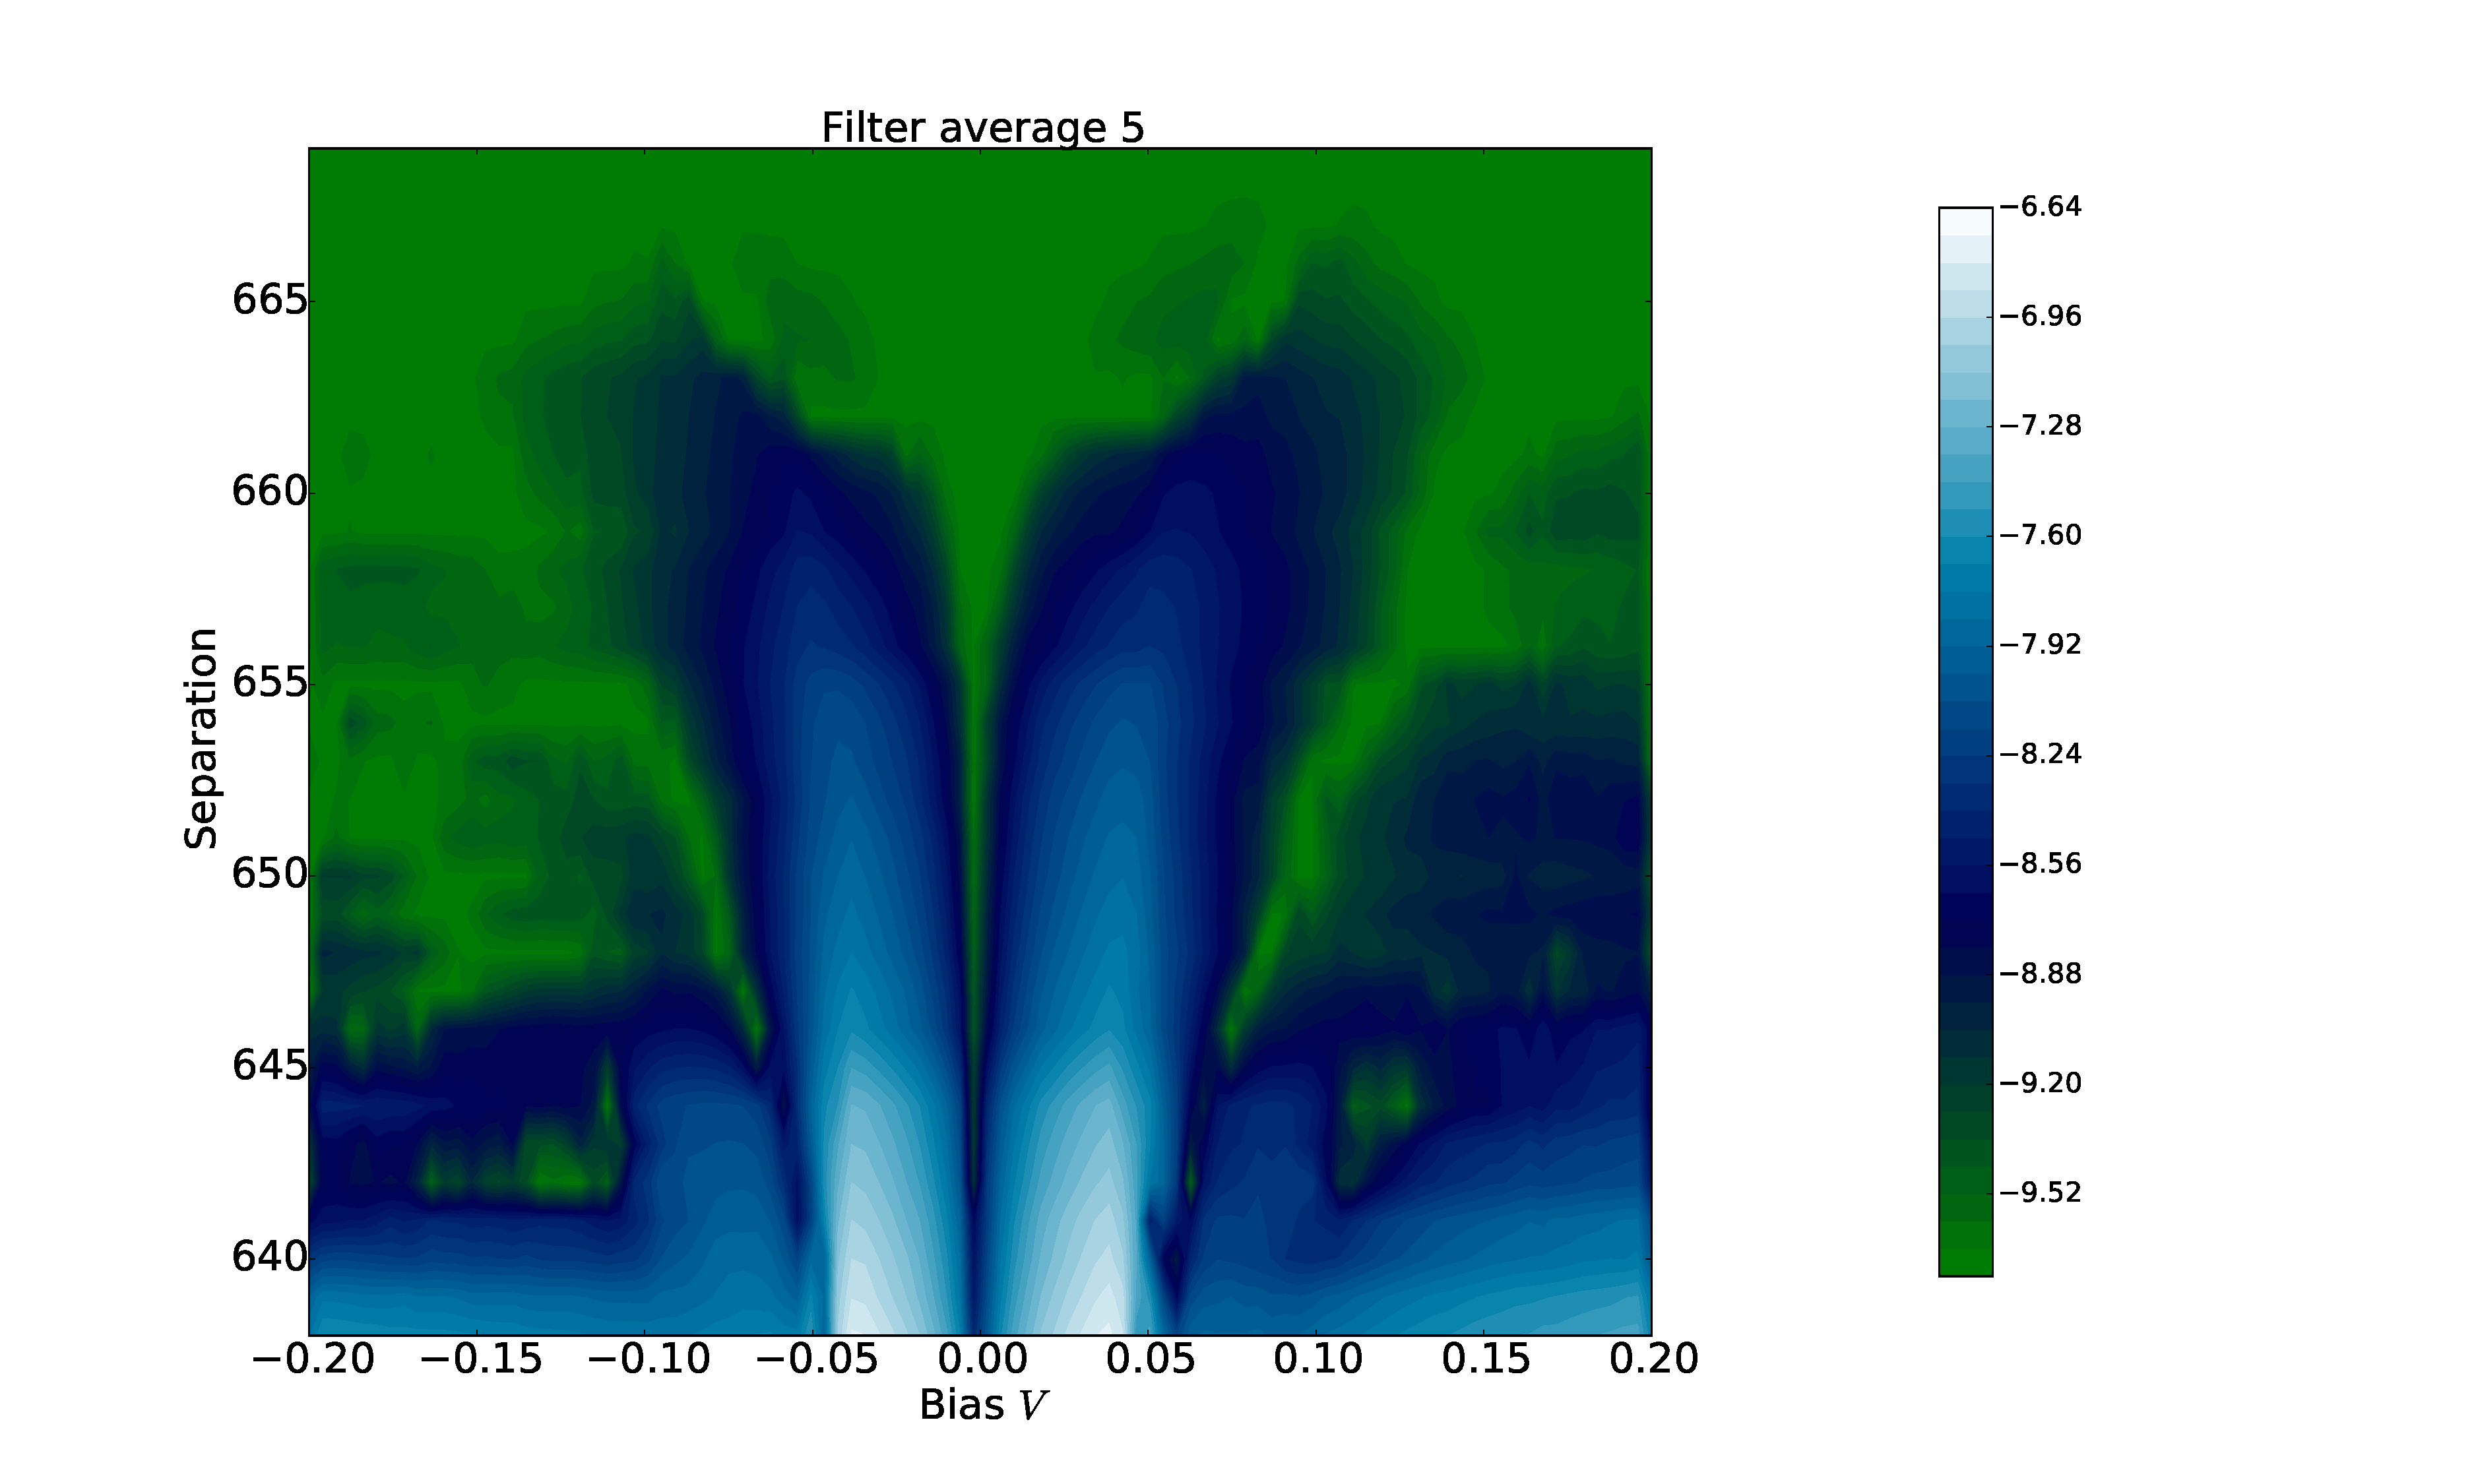
\includegraphics[width=.99\textwidth,clip=true, trim=4cm 0cm 10cm 4cm]{pdf/perrin_experiment_abs.pdf}
    \caption{Experimental data by \citet{perrinnano}, the colours are proportional to $^{10}\text{log}\left|I(V)\right|$. As elsewhere, $I(V) = -I(-V)$. The current is capped at the lower end to $10^{-10}$ A.}
    \label{fig:perrindata}
\end{figure}

Next, I want to presents a few results that show clearly that the new theory is in better quantitative agreement with the results by \citet{perrinnano}. However, the current landscape at different parameters does not change smoothly, which makes it troublesome to \emph{fit} the predicted smoothly. Instead, I performed an automatic rough parameter scan and selected results manually.

In particular, I have taken care to select results both in the first and second charge state, to show that both possibilities are relevant. First, I want to discuss the spinless results and then the spinfull results. For all of these figures, $\alpha=0.400$, $\Gamma=0.010$, $\tau=0.010$ unless otherwise noted. The experimental current is measured in the exact same way as Figure~\ref{fig:perrindata}, but only the (near) blockade-free region was used.

Figure~\ref{fig:fitspinless5} with $U=0.30$ and $\epsilon_0=-0.30$, shows a very clear NDC with maximum current within a factor of two relative to the averaged experimental current, a significant improvement over the previous prefactor $10^-5$ in Ref.~\cite{perrinnano}.


\begin{figure}[htb]
    \centering
    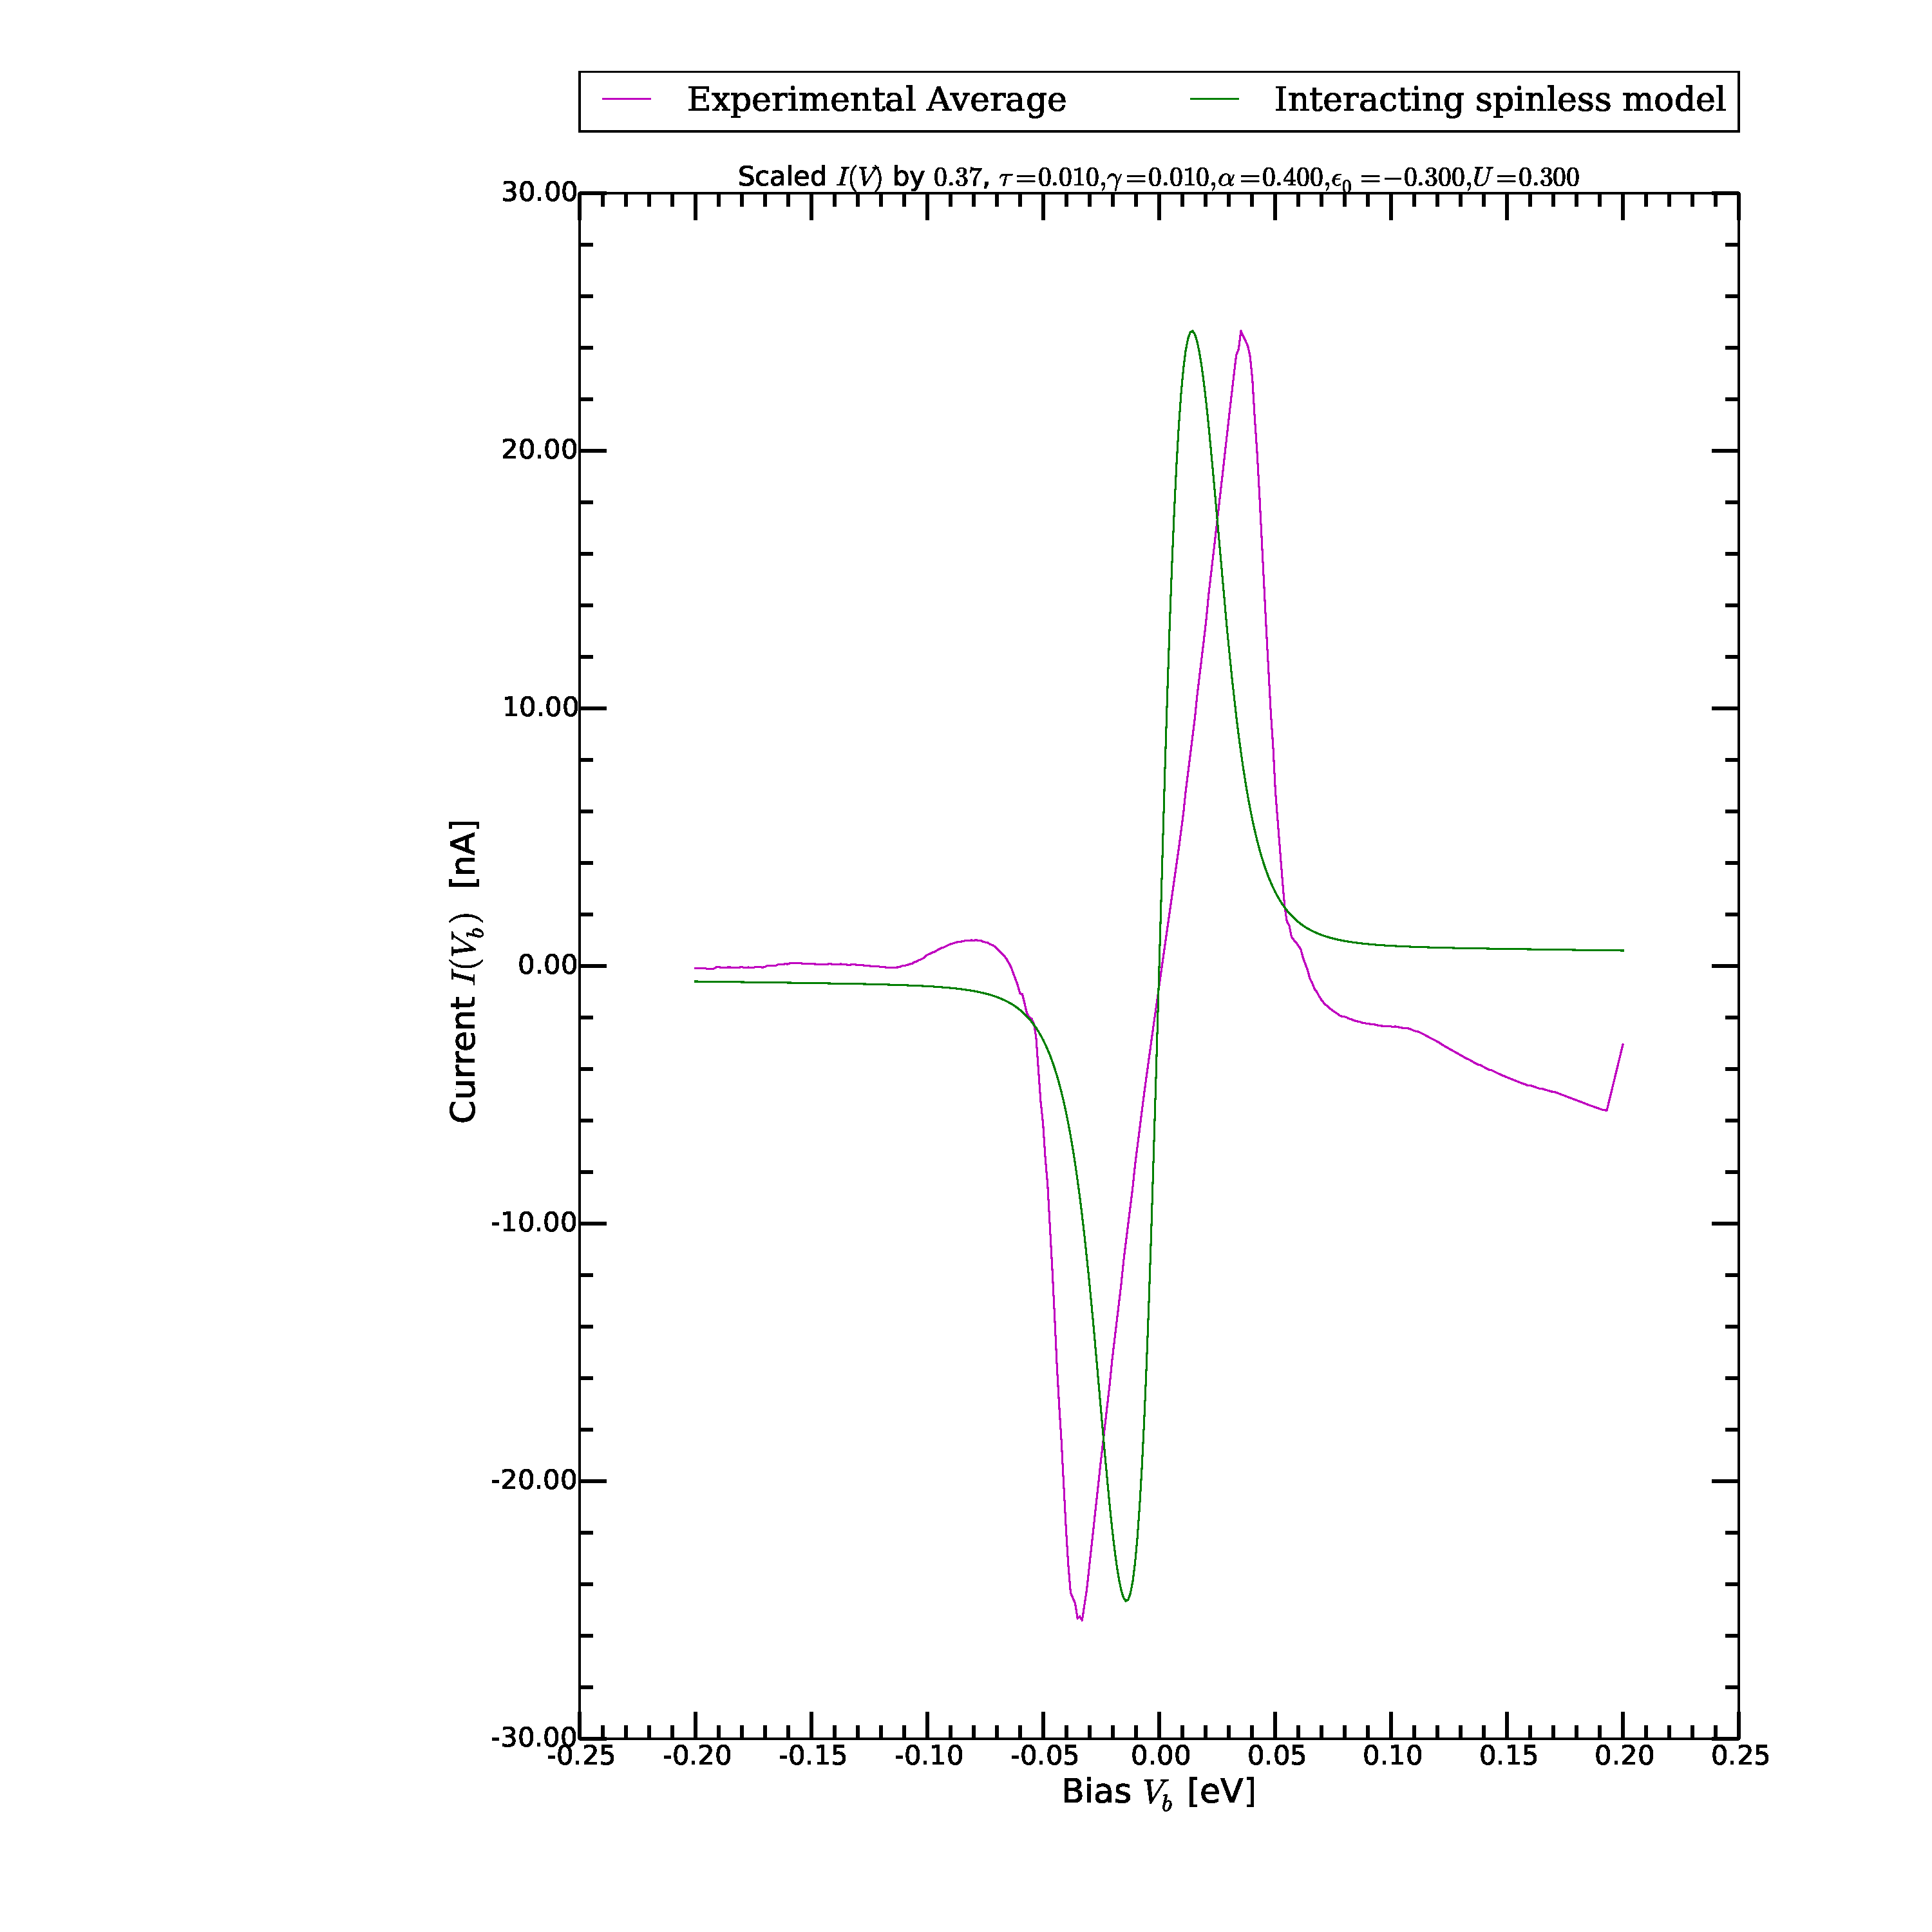
\includegraphics[width=.95\textwidth, clip=true, trim=11cm 2cm 2cm 0cm]{pdf/fit/fit_spinless_5.pdf}
    \caption{Experimental $I(V)$ (Magenta) versus calculated spinless current $I(V)$ (green). In this figure, $U=0.30$ and $\epsilon_0 = -0.30$. The current is scaled by $0.37$ so that it has the same peak height as the experimental current.}
    \label{fig:fitspinless5}
\end{figure} 
\begin{figure}[htb]
    \centering
    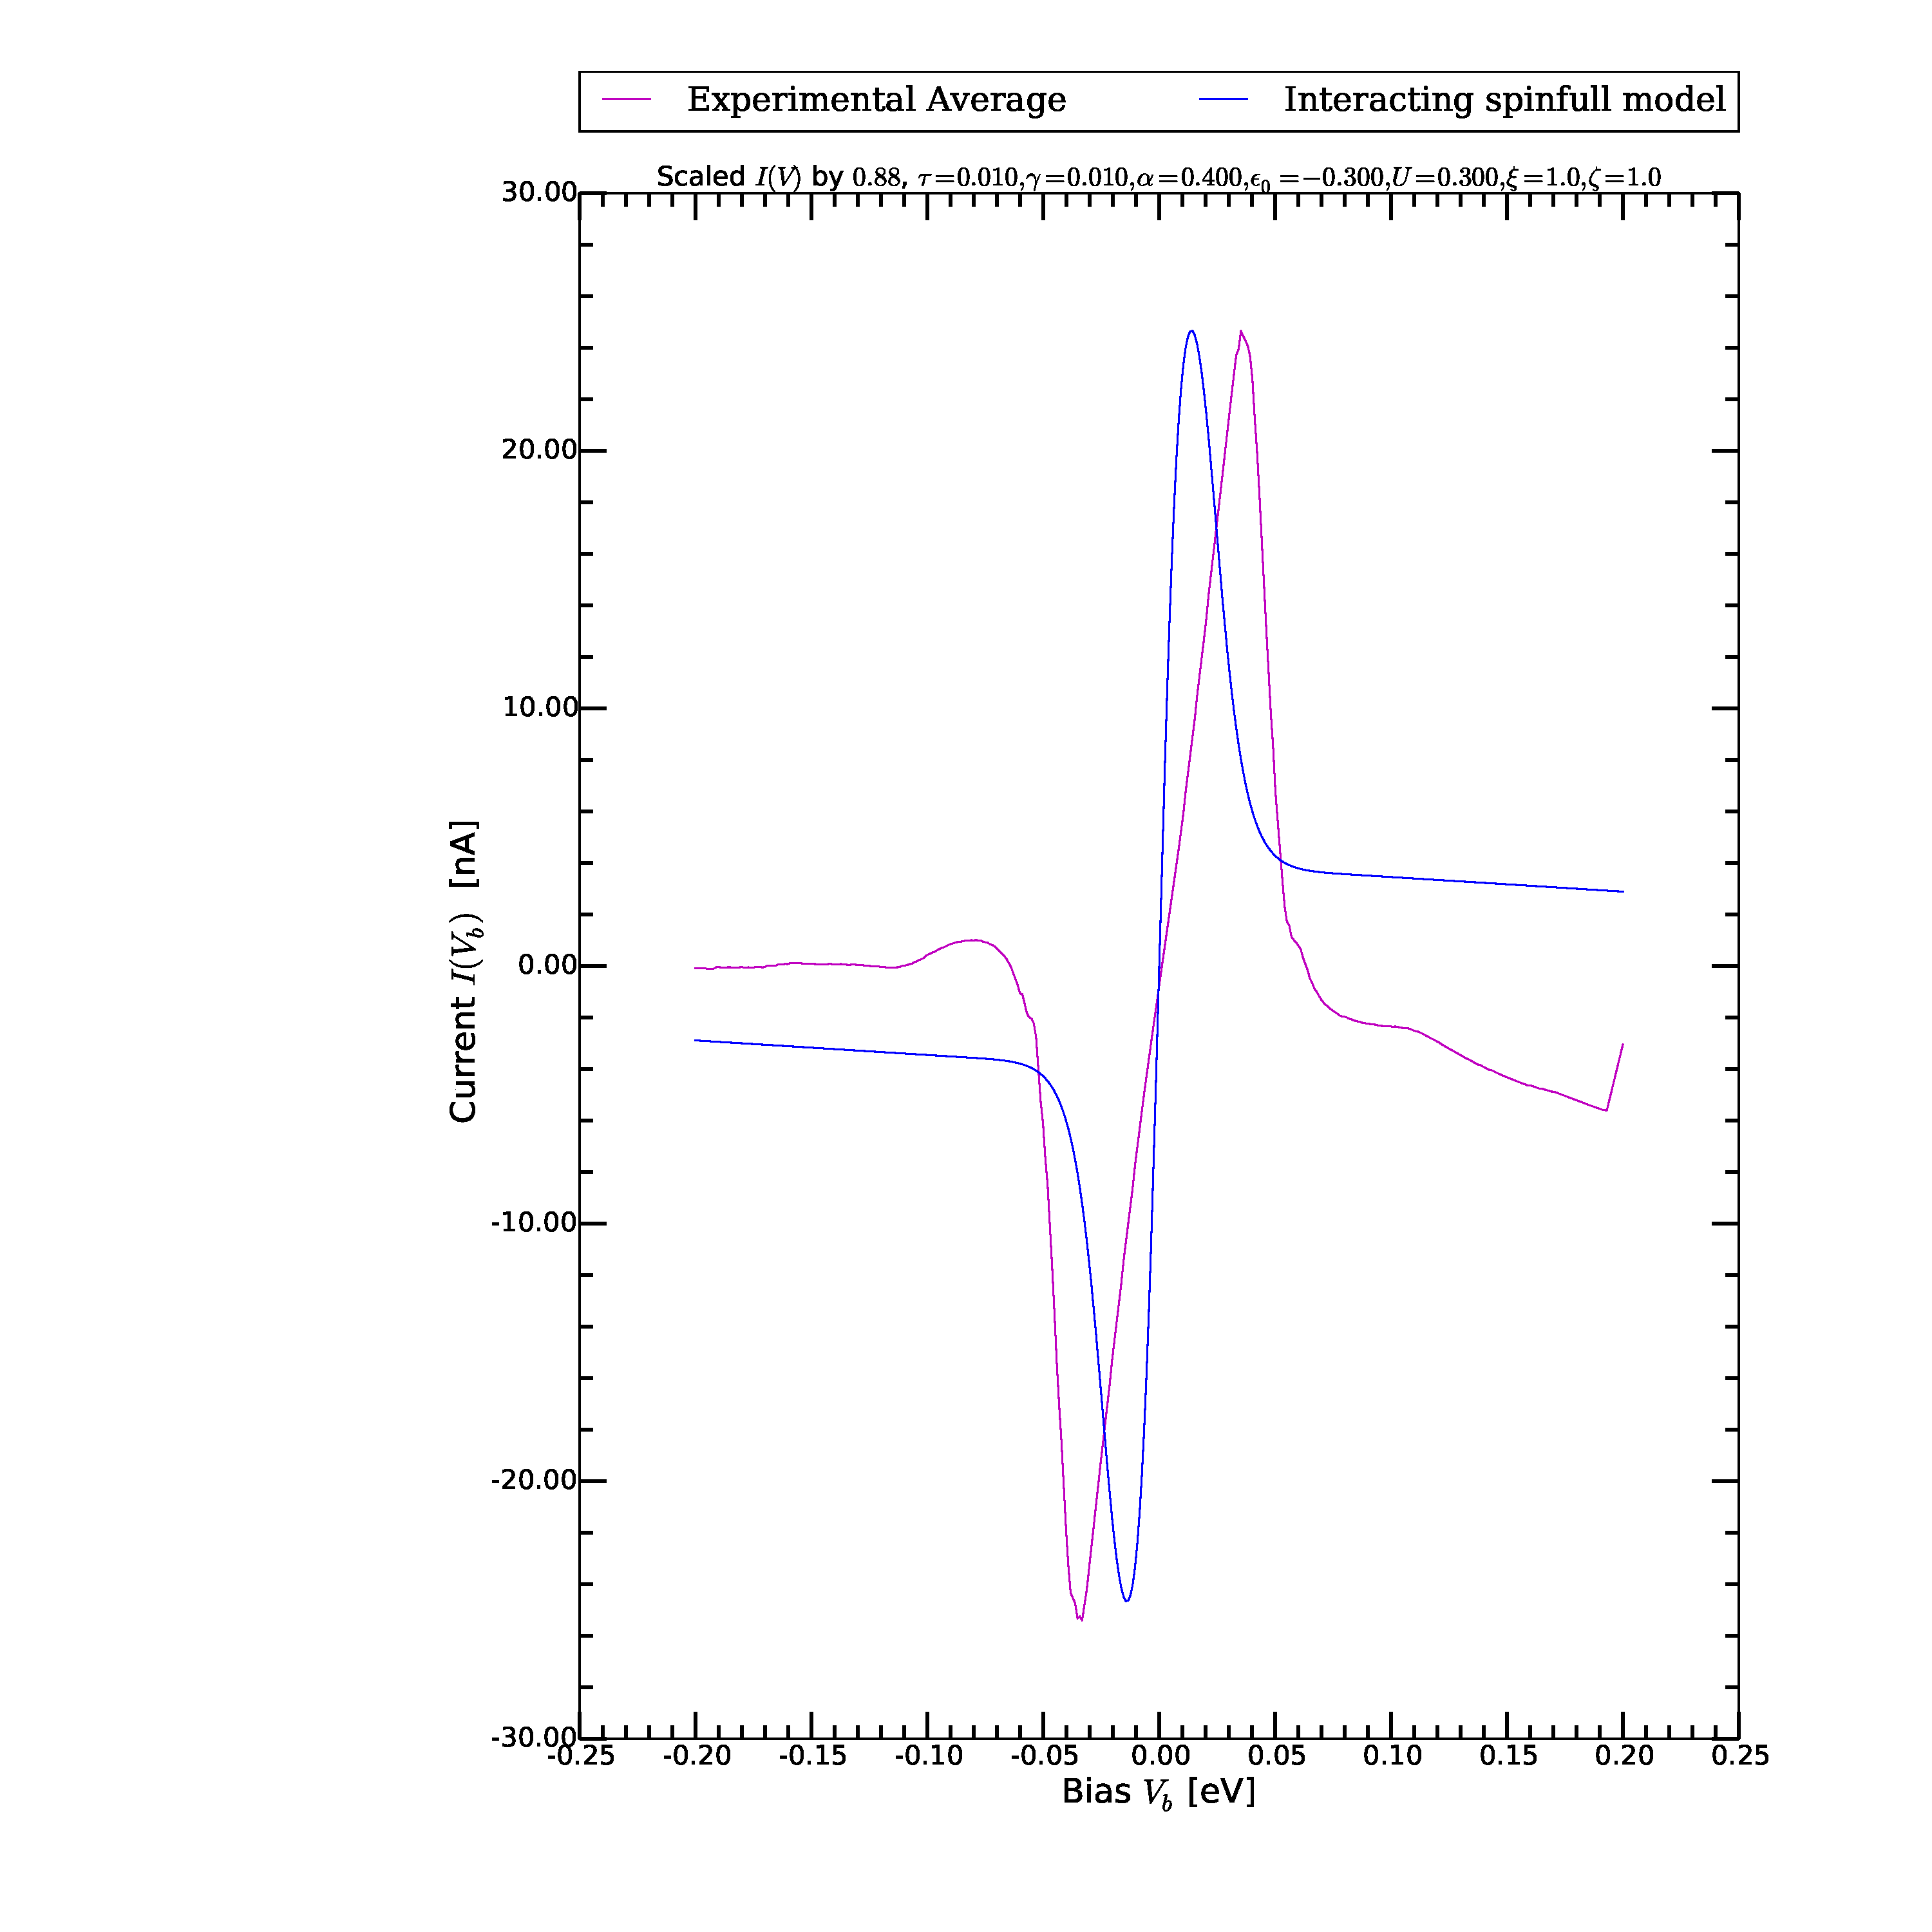
\includegraphics[width=.95\textwidth, clip=true, trim=11cm 2cm 2cm 0cm]{pdf/fit/fit_spinfull_1.pdf}
    \caption{Experimental $I(V)$ (Magenta) versus calculated spinfull current $I(V)$ (green). In this figure, $U=0.30$ and $\epsilon_0 = -0.30$. The current is scaled by $0.88$ so that it has the same peak height as the experimental current.}
    \label{fig:fitspinfull1}
\end{figure} 

The second charge state is shown in Figure~\ref{fig:fitspinfull1}, which does have lower peak current, within a factor 2 of the experimental average. For $U=0.50$, the first charge state is very similar to the second, but is at $169$ \% while the second charge state is at $95$ \% of the experimental average.

To conclude, the quantitative agreement with \citet{perrinnano} is significantly improved in the first and second charge states. While the peak voltages do not exactly agree, we only performed a very limited rough scan of the parameter space. I am confident that the parameters can be tuned for better qualitative agreement, but could not do so due to time-constraints.

\section{Self-Consistent Results}
\label{sec:resultsselfconsistencycalc}

\begin{figure}[htb]
    \centering
    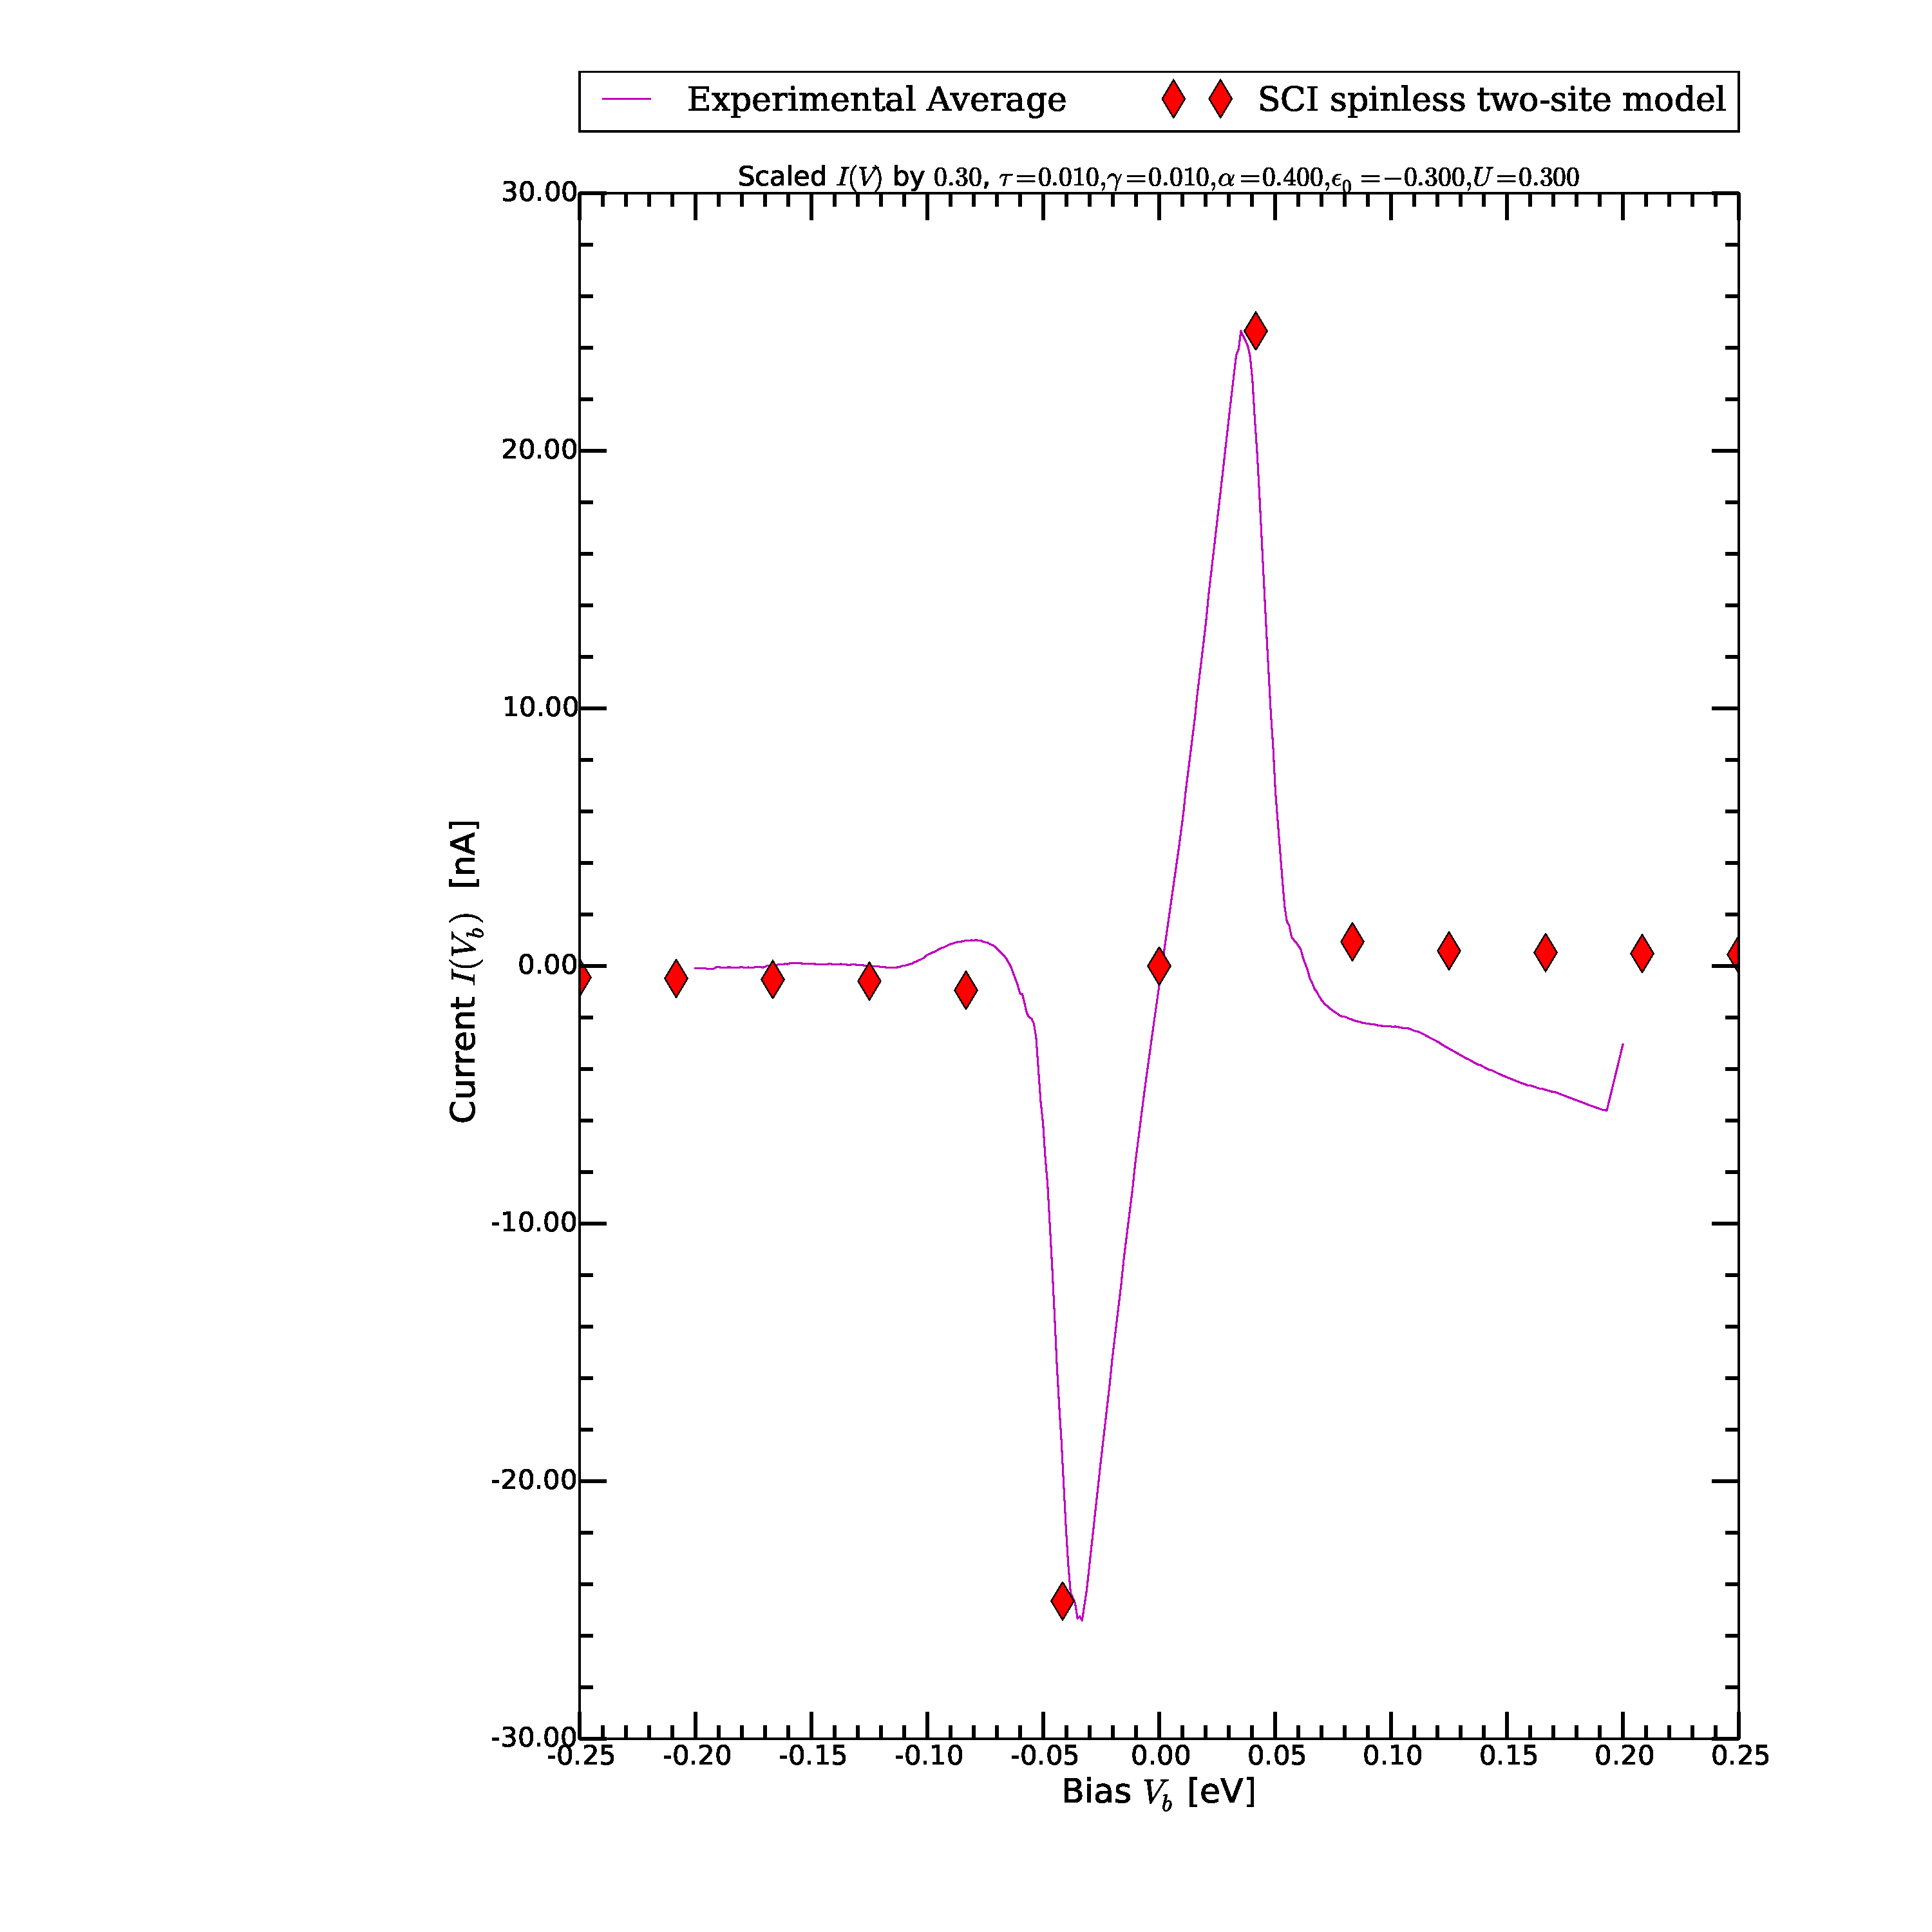
\includegraphics[width=.95\textwidth, clip=true, trim=11cm 2cm 2cm 0cm]{pdf/selfconsistent_fit_current_0.pdf}
    \caption{ }
    \label{fig:figselfconsistent}
\end{figure} 

%clearpage dumps all images in the stack. Also prevents images from skipping chapters.
\clearpage
\references{dissertation}